\pdfoutput=1
\documentclass[a4paper,english,fleqn,11pt,final]{scrartcl}


\usepackage[utf8]{inputenc}
\usepackage[T1]{fontenc}
\usepackage{lmodern}
\usepackage[english]{babel}

\usepackage[protrusion=true,expansion=true,final]{microtype}
\usepackage{textcomp}

\usepackage{xcolor}
\usepackage[heavycircles]{stmaryrd}
\usepackage[centertags,sumlimits,intlimits,namelimits,fleqn]{amsmath}
\usepackage[fixamsmath,disallowspaces]{mathtools}
\usepackage{bussproofs}
\usepackage{lplfitch}

\usepackage{relsize}
\usepackage{scalerel}

\usepackage{braket}

\usepackage{amsfonts}
\usepackage{amssymb}

\usepackage[backref=none,pagebackref=false,hyperindex=true,hyperfootnotes=false,bookmarks=true,pdfpagelabels=true,final]{hyperref}

\hypersetup{
    colorlinks,
    linkcolor={red!80!black},
    citecolor={blue!50!black},
    urlcolor={blue!80!black}
}


\usepackage{amsthm}


\usepackage[babel,autostyle=true,strict]{csquotes}
\MakeOuterQuote{"}
\usepackage[xspace]{ellipsis}
\usepackage[section]{placeins} 

\usepackage{bookmark}
\usepackage{pdfcolmk} 
\usepackage{authblk}

\hypersetup{
    colorlinks,
    linkcolor={red!50!black},
    citecolor={blue!50!black},
    urlcolor={blue!80!black}
}

\usepackage{tabularx}
\usepackage{booktabs}


\usepackage{tikz}
\usepackage{pgf}
\usetikzlibrary{arrows,positioning}
\usetikzlibrary{shapes.geometric}
\usetikzlibrary{decorations.pathreplacing}

\newcommand{\TODO}[1]{\textbf{\color{red}TODO: #1}\xspace}



\DeclareMathOperator*{\bigand}{\prod}
\DeclareMathOperator*{\bigor}{\sum}

\newcommand{\ie}{i.e.\@\xspace}
\newcommand{\eg}{e.g.\@\xspace}
\newcommand{\wrt}{w.\,r.\,t.\@\xspace}
\newcommand{\suchthat}{s.\,t.\@\xspace}
\newcommand{\fa}{f.\,a.\@\xspace}
\newcommand{\wloss}{w.l.o.g.\@\xspace}
\newcommand{\Wloss}{W.l.o.g.\@\xspace}

\newcommand{\numberClassFont}[1]{\mathbb{#1}}     
\newcommand{\logicClFont}[1]{\mathcal{#1}}        
\newcommand{\logicOpFont}[1]{\mathsf{#1}}         
\newcommand{\mathCommandFont}[1]{\mathrm{#1}}     

\newcommand{\size}[1]{{\protect\ensuremath{\vert\nobreak#1\nobreak\vert}}}
\newcommand{\pow}[1]{{\protect\ensuremath{\mathord{\mathfrak{P}(\nobreak#1\nobreak)}}}}
\newcommand{\arity}[1]{{\protect\ensuremath{\mathCommandFont{ar}(#1)}}}
\newcommand{\Mod}[1]{{\protect\ensuremath{\mathsf{Mod}(#1)}}}
\newcommand{\N}{\protect\ensuremath{\numberClassFont{N}}\xspace}


\newcommand{\negg}{{\sim}}
\newcommand{\depop}{{=\!\!(\cdot,\cdot)}}
\newcommand{\dep}[1]{{=\!\!(#1)}}
\newcommand{\depopp}{\depop}

\newcommand{\PROP}{\protect\ensuremath\logicOpFont{PROP}}

\newcommand{\logic}[1]{\ensuremath{\mathsf{#1}}\xspace}


\newcommand{\PS}{\logic{Prop}}
\newcommand{\D}{\logic{D}}
\newcommand{\PL}{\logic{PL}}
\newcommand{\QPL}{\logic{QPL}}
\newcommand{\QPPL}{\logic{(Q)PL}}
\newcommand{\ML}{\logic{ML}}
\newcommand{\FO}{\logic{FO}}
\newcommand{\SO}{\logic{SO}}
\newcommand{\IF}{\logic{IF}}

\newcommand{\PTL}{\logic{PTL}}
\newcommand{\QPDL}{\logic{QPDL}}
\newcommand{\PDL}{\logic{PDL}}
\newcommand{\QPTL}{\logic{QPTL}}
\newcommand{\QPPTL}{\logic{(Q)PTL}}
\newcommand{\MTL}{\logic{MTL}}
\newcommand{\TL}{\logic{TL}}
\newcommand{\MDL}{\logic{MDL}}
\newcommand{\EMDL}{\logic{EMDL}}
\newcommand{\EEMDL}{\logic{(E)MDL}}
\newcommand{\QPD}{\logic{QBD}}
\newcommand{\MINC}{\logic{MInc}}
\newcommand{\MINCEX}{\logic{MIncEx}}
\newcommand{\QPINC}{\logic{QPInc}}
\newcommand{\QPINCEX}{\logic{QPIncEx}}
\newcommand{\PINCEX}{\logic{PIncEx}}
\newcommand{\PINC}{\logic{PInc}}
\newcommand{\QPIND}{\logic{QPIL}}
\newcommand{\QPIL}{\logic{QPIL}}
\newcommand{\PIND}{\logic{PIL}}
\newcommand{\PIL}{\logic{PIL}}
\newcommand{\MIL}{\logic{MIL}}

\newcommand{\NE}{\text{\textsc{ne}}}
\newcommand{\E}{\protect\ensuremath\logicOpFont{E}}

\newcommand{\Fr}{\mathrm{Fr}}
\newcommand{\Var}{\mathrm{Var}}

\newcommand{\frakA}{\protect\ensuremath{\mathfrak{A}}}
\newcommand{\frakB}{\protect\ensuremath{\mathfrak{B}}}
\newcommand{\frakC}{\protect\ensuremath{\mathfrak{C}}}
\newcommand{\frakD}{\protect\ensuremath{\mathfrak{D}}}
\newcommand{\frakK}{\protect\ensuremath{\mathfrak{K}}}
\newcommand{\calA}{\protect\ensuremath{\mathcal{A}}}
\newcommand{\calB}{\protect\ensuremath{\mathcal{B}}}
\newcommand{\calC}{\protect\ensuremath{\mathcal{C}}}
\newcommand{\calD}{\protect\ensuremath{\mathcal{D}}}
\newcommand{\calF}{\protect\ensuremath{\mathcal{F}}}
\newcommand{\calG}{\protect\ensuremath{\mathcal{G}}}
\newcommand{\calH}{\protect\ensuremath{\mathcal{H}}}
\newcommand{\calI}{\protect\ensuremath{\mathcal{I}}}
\newcommand{\calL}{\protect\ensuremath{\mathcal{L}}}
\newcommand{\calK}{\protect\ensuremath{\mathcal{K}}}
\newcommand{\calM}{\protect\ensuremath{\mathcal{M}}}
\newcommand{\calO}{\protect\ensuremath{\mathcal{O}}}
\newcommand{\calP}{\protect\ensuremath{\mathcal{P}}}
\newcommand{\calQ}{\protect\ensuremath{\mathcal{Q}}}
\newcommand{\calS}{\protect\ensuremath{\mathcal{S}}}
\newcommand{\calT}{\protect\ensuremath{\mathcal{T}}}
\newcommand{\calU}{\protect\ensuremath{\mathcal{U}}}
\newcommand{\calV}{\protect\ensuremath{\mathcal{V}}}
\newcommand{\calX}{\protect\ensuremath{\mathcal{X}}}
\newcommand{\sfD}{\protect\ensuremath{\mathsf{D}}}
\newcommand{\sfS}{\protect\ensuremath{\mathsf{S}}}
\newcommand{\sfH}{\protect\ensuremath{\mathsf{H}}}
\newcommand{\sfK}{\protect\ensuremath{\mathsf{K}}}
\newcommand{\sfL}{\protect\ensuremath{\mathsf{L}}}
\newcommand{\sfM}{\protect\ensuremath{\mathsf{M}}}
\newcommand{\sfQ}{\protect\ensuremath{\mathsf{Q}}}
\newcommand{\sfU}{\protect\ensuremath{\mathsf{U}}}
\newcommand{\sfB}{\protect\ensuremath{\mathsf{B}}}
\newcommand{\sfT}{\protect\ensuremath{\mathsf{T}}}
\newcommand{\sfO}{\protect\ensuremath{\mathsf{O}}}

\providecommand{\dfn}{\mathrel{\mathop:}=}
\providecommand{\ddfn}{\mathrel{\mathop{{\mathop:}{\mathop:}}}=}

\newcommand{\imp}{\rightarrow}
\newcommand{\limp}{\multimap}
\newcommand{\timp}{\rightarrowtriangle}
\newcommand{\ltimp}{\leftarrowtriangle}
\newcommand{\tequiv}{\leftrightarrowtriangle}
\newcommand{\equ}{\leftrightarrow}
\newcommand{\eqpr}{\dashv\vdash}
\newcommand{\tens}{\otimes}
\newcommand{\frakM}{\mathfrak{M}}
\newcommand{\Deriv}[1]{{\normalfont\textsf{#1}}}
\newcommand{\Apply}[1]{\textsf{\scriptsize{}#1}}
\newenvironment{bprooftree}{\leavevmode\hbox\bgroup}{\DisplayProof\egroup}

\newcommand{\rel}{\mathsf{rel}}

\newcommand{\oland}{\owedge}

\DeclareMathOperator*{\bigovee}{\scalerel*{\ovee}{\sum}}
\DeclareMathOperator*{\bigoland}{\scalerel*{\owedge}{\sum}}
\DeclareMathOperator*{\bigowedge}{\scalerel*{\owedge}{\sum}}
\DeclareMathOperator*{\bigtens}{\bigotimes}
\DeclareMathOperator*{\bigdiamond}{\scalerel*{\Diamond}{\sum}}

\DeclareMathOperator{\shriek}{!}
\DeclareMathOperator{\indep}{\perp}
\DeclareMathOperator{\inclusion}{\subseteq}
\DeclareMathOperator{\exclusion}{\mid}

\EnableBpAbbreviations

\newcommand{\falsum}{\mathrlap{\,\bot}\bot\,}
 
\theoremstyle{plain}
\newtheorem{theorem}{Theorem}[section]

\newtheorem{proposition}[theorem]{Proposition}
\newtheorem{lemma}[theorem]{Lemma}
\newtheorem{corollary}[theorem]{Corollary}
\theoremstyle{definition}
\newtheorem{definition}[theorem]{Definition}
\newtheorem{example}[theorem]{Example}

\makeatletter
\newtheorem*{rep@theorem}{\rep@title}
\newcommand{\newreptheorem}[2]{
\newenvironment{rep#1}[1]{
 \def\rep@title{#2 \ref{##1}}
 \begin{rep@theorem}}
 {\end{rep@theorem}}}
\makeatother
\newreptheorem{proposition}{Proposition}
\newreptheorem{lemma}{Lemma}
\newreptheorem{theorem}{Theorem}


\newcommand{\thm}{\text{\scriptsize\; (thm)}}

\usepackage[backend=biber,style=numeric,sortcites,url=false,maxbibnames=99,maxcitenames=2,citetracker=true]{biblatex}



\DeclareFieldFormat[article]{title}{\mkbibemph{#1}}
\DeclareFieldFormat[article]{journal}{#1}
\DeclareFieldFormat[article]{journaltitle}{#1}
\DeclareFieldFormat[article]{volume}{\textbf{#1}}
\DeclareFieldFormat[article]{number}{no.~#1}



\DeclareFieldFormat[incollection]{title}{\mkbibemph{#1}}
\DeclareFieldFormat[incollection]{booktitle}{#1}
\DeclareFieldFormat[incollection]{volume}{\textbf{#1}}
\DeclareFieldFormat[incollection]{number}{(#1)}




\DeclareFieldFormat[inproceedings]{title}{\mkbibemph{#1}}
\DeclareFieldFormat[inproceedings]{booktitle}{#1}
\DeclareFieldFormat[inproceedings]{volume}{\textbf{#1}}
\DeclareFieldFormat[inproceedings]{number}{(#1)}


\DeclareFieldFormat[unpublished]{title}{\mkbibemph{#1}}


\DeclareFieldFormat[thesis]{title}{\mkbibemph{#1}}


\renewcommand*{\finalnamedelim}{\addcomma\space}
\renewcommand*{\finalnamedelim}{\addspace\bibstring{and}\space}

\renewbibmacro*{volume+number+eid}{
  \printfield{volume}\space
  \printtext[parens]{\usebibmacro{date}}
  \setunit{\addcomma\space}
  \printfield{number}
  \setunit{\addcomma\space}
  \printfield{eid}
  }


\renewbibmacro*{issue+date}{
  \iffieldundef{issue}
      {}
      {\printfield{issue}}
  \newunit}

\renewbibmacro{in:}{}
 
\makeatletter
\DeclareOldFontCommand{\rm}{\normalfont\rmfamily}{\mathrm}
\DeclareOldFontCommand{\sf}{\normalfont\sffamily}{\mathsf}
\DeclareOldFontCommand{\tt}{\normalfont\ttfamily}{\mathtt}
\DeclareOldFontCommand{\bf}{\normalfont\bfseries}{\mathbf}
\DeclareOldFontCommand{\it}{\normalfont\itshape}{\mathit}
\DeclareOldFontCommand{\sl}{\normalfont\slshape}{\@nomath\sl}
\DeclareOldFontCommand{\sc}{\normalfont\scshape}{\@nomath\sc}
\makeatother

\title{Axiomatizations of Team Logics}
\author{Martin Lück}
\date{\vspace{-5ex}}
\affil{\small{}Leibniz Universität Hannover, Institut für Theoretische Informatik,\\
Appelstraße 4, 30167 Hannover, Germany\\\texttt{lueck@thi.uni-hannover.de}}


\bibliography{axiom}

\begin{document}
\maketitle

\begin{abstract}
\textbf{Abstract.}
In a modular approach, we lift Hilbert-style proof systems for propositional, modal and first-order logic to generalized systems for their respective team-based extensions.
We obtain sound and complete axiomatizations for the dependence-free fragment FO() of Väänänen's first-order team logic TL, for propositional team logic PTL, quantified propositional team logic QPTL, modal team logic MTL, and for the corresponding logics of dependence, independence, inclusion and exclusion.

As a crucial step in the completeness proof, we show that the above logics admit, in a particular sense, a semantics-preserving elimination of modalities and quantifiers from formulas.
\end{abstract}

\noindent\textit{Keywords and phrases:} axiomatization, dependence logic, propositional team logic, modal team logic, team logic

\noindent\textit{1998 ACM Subject Classification:} F.4.1 Mathematical Logic


\section{Introduction}

While their history goes back to ancient philosophers, propositional and modal logics have assumed an outstanding role in the age of modern computer science, with plentiful applications in software verification, modeling, artificial intelligence, and protocol design.
An important property of a logical framework is \emph{completeness}, \ie, that the act of mechanical reasoning can effectively be done by an algorithm.
The question of completeness of first-order logic, which is the foundation of today's mathematics, was not settled until the famous result of Gödel in 1929.
Until today, the area of proof theory has achieved tremendous progress and is still a growing field, especially with regard to many variants of propositional and modal logics as well as non-classical logics (see \eg Fitting \cite{fitting_proof_1983}).

\smallskip

A recent extension of classical logics is so-called \emph{team logic}.
It originated from the concept of quantifier dependence and independence. The following question has been long-known in linguistics: how can the statement
\begin{quote}
\emph{For every  there is , and for every  there is  such that P(x,y,u,v).}
\end{quote} be formalized in first-order logic such that  and  are chosen independently?
Some suggestions were Henkin's \emph{branching quantifiers} \cite{Henkin1961} as well as \emph{in\-de\-pend\-ence-friendly logic}  by Hintikka and Sandu~\cite{hintikka_informational_1989}.
The idea of the latter is to assert dependence and independence between quantifiers syntactically, implemented semantically by a game of imperfect information.
Hodges \cite{Hodges1997} proved that  also admits a compositional semantics if formulas were evaluated on \emph{teams}, which are sets of assignments, instead of single assignments.
In this vein, Väänänen~\cite{vaananen_dependence_2007} introduced \emph{dependence logic} .
Here, the fundamental idea is that dependencies are not stated alongside the quantifiers, but instead are expressed as logical \emph{dependence atoms}, written , which means " functionally determines ."

\smallskip

Beside Väänänen's dependence atom, a variety of atomic formulas solely for reasoning in teams were introduced. Galliani~\cite{galliani_inclusion_2012} as well as Grädel and Väänänen~\cite{gradel2013dependence} pointed out connections to database theory; they formalized common constraints like \emph{independence} , \emph{inclusion}  and \emph{exclusion}  as atoms in the framework of team semantics.
Beside first-order logic, all these atoms have also been adapted for modal logic  \cite{vaananen_modal_2008}, and (quantified) propositional logic  resp.\  \cite{sano_et_al,yang_propositional_2016,gandalf}.

\smallskip

As for any logic, the question of axiomatizability arises for these logics with team semantics, in particular for the extensions of first-order logic.
However, dependence logic  is as expressive as existential second-order logic  \cite{vaananen_dependence_2007}, while its extension , obtained from  by adding a semantical negation , is equivalent to full second-order logic  \cite{hutchison_team_2009}.
Accordingly, both are non-axiomatizable.
Later, Kontinen and Väänänen~\cite{kontinen_axiomatizing_2013} gave a partial axiomatization in the sense that -consequences of -formulas are derivable, and recently a system that can derive all so-called \emph{negatable} -formulas was presented by Yang~\cite{Yang2016}.

\smallskip

For certain fragments of propositional and modal team logic, axiomatizations exist.
Hannula~\cite{Hannula16} presented natural deduction systems for propositional dependence logic , quantified propositional dependence logic  and extended modal dependence logic .
By contrast, Sano and Virtema~\cite{sano_et_al} gave Hilbert-style axiomatizations and labeled tableau calculi for propositional dependence logic  and (extended) modal dependence logic .
Independently, Yang~\cite{Yang17} presented both Hilbert-style axiomatizations and natural deduction systems for a family of so-called \emph{downward-closed} modal logics with team semantics, which includes  as well.

However, a fundamental restriction of these solutions is that they all rely on the absence of Boolean negation.
As a consequence, team logics with negation, most notably propositional team logic (), modal team logic () and , require a different approach.

\smallskip

\subsubsection*{Contribution}

In this paper, we present complete axiomatizations for several team logics including the -free fragment of , coined  by Gallani~\cite{Galliani14}.
Here, we consider it under \emph{lax semantics}~\cite{galliani_inclusion_2012}.

By showing that  is axiomatizable, we identify the dependence atom , and not team semantics itself, as the source of incompleteness of  and .
One interpretation is that reasoning about teams can be axiomatized; but only if we cannot talk about the internal dependencies between the elements of the team.

A crucial step in the completeness proof is the perhaps surprising fact that  without  collapses to , the Boolean closure of classical first-order logic  under team semantics.
The latter has the so-called \emph{flatness property}, which implies that any classical proof system of  is also adequate for team semantics.
From there, an axiomatization of  is easily found in a similar way as for propositional logic.

Whether logics not collapsing to  have axiomatizations is beyond the scope of this paper.
Our approach, however, also yields results for (quantified) propositional and modal team logics.
They can define their atoms of dependence, independence and inclusion in terms of other connectives, whereas this is not possible in the first-order setting.
For this reason, the logics ,  and  collapse to ,  and  in a similar fashion as  to , and we obtain complete axiomatizations as a byproduct.
Figure~\ref{fig:overview} illustrates this.


\smallskip

The article is organized as follows.
Let us remark that the axiomatizations as a whole can be found in Figure~\ref{fig:all-axioms}.
In each section of the paper, one subsystem is introduced.
First, the system  is presented in Section~\ref{sec:boolean} as a complete proof system for the Boolean closure  under team semantics, where .
In Section~\ref{sec:splitting}, the system  is added which permits to eliminate the \emph{splitting disjunction}  in a semantics-preserving manner.
By means of this elimination,  collapses to  in the proof system.
Likewise, in Section~\ref{sec:modal} it is shown that modalities can be eliminated in a system we call , and that the problem of the axiomatization of  is thereby reduced to that of  as well.
The results on  and  were presented earlier \cite{csl16axiom}, and are now extended to logics containing quantifiers, namely quantified Boolean formulas and first-order logic.
Section~\ref{sec:qbf} introduces the system  which allows to axiomatize and hence eliminate quantifiers in a similar fashion as the modalities.


\begin{figure}\centering
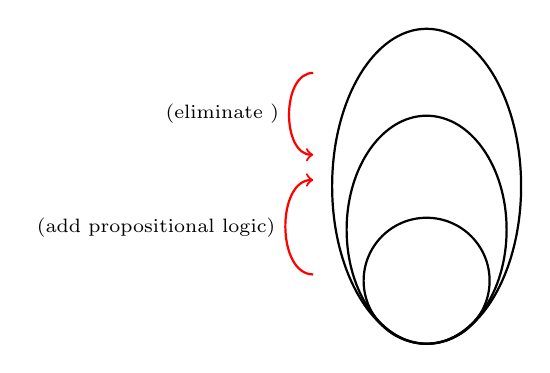
\begin{tikzpicture}[thick,scale=0.8]
\draw (0,-.3) ellipse (1.5cm and 2.5cm);
\node (MTL) at (0,1.8cm){};
\node[color=red] at (0,1.2cm) {};
\draw (0,-0.99cm) ellipse (1.27cm and 1.81cm);
\node (BML) at (0,0.2cm){};
\node[color=red] at (0,-.4cm) {};
\draw (0,-1.8cm) ellipse (1cm and 1cm);
\node (ML) at (0,-1.8cm){};
\node[color=red] at (0.1cm,-2.4cm) {};
\draw[red,<-] (-1.8cm,0.2cm) to[in=180,out=180] node[left,black]{\scriptsize(eliminate )} (-1.8cm,1.5cm);
\draw[red,->] (-1.8cm,-1.7cm) to[in=180,out=180] node[left,black]{\scriptsize(add propositional logic)} (-1.8cm,-.2cm);
\end{tikzpicture}
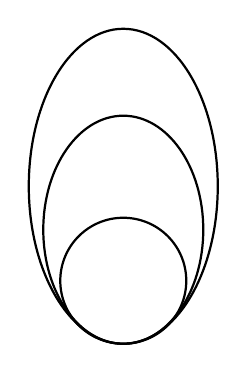
\begin{tikzpicture}[thick,scale=0.8]
\draw (0,-.3) ellipse (1.5cm and 2.5cm);
\node (MTL) at (0,1.8cm){};
\node[color=red] at (0,1.2cm) {};
\draw (0,-0.99cm) ellipse (1.27cm and 1.81cm);
\node (BML) at (0,0.2cm){};
\node[color=red] at (0,-.4cm) {};
\draw (0,-1.8cm) ellipse (1cm and 1cm);
\node (ML) at (0,-1.8cm){};
\node[color=red] at (0.1cm,-2.4cm) {};
\end{tikzpicture}
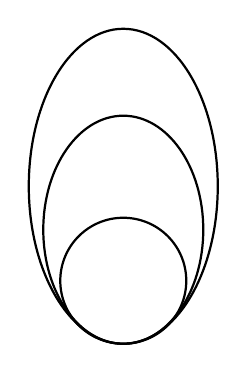
\begin{tikzpicture}[thick,scale=0.8]
\draw (0,-.3) ellipse (1.5cm and 2.5cm);
\node (MTL) at (0,1.75cm){};
\node[color=red] at (0,1.2cm) {};
\draw (0,-0.99cm) ellipse (1.27cm and 1.81cm);
\node (BML) at (0,0.2cm){};
\node[color=red] at (0,-.4cm) {};
\draw (0,-1.8cm) ellipse (1cm and 1cm);
\node (ML) at (0,-1.8cm){};
\node[color=red] at (0cm,-2.4cm) {};
\end{tikzpicture}
\caption{Lower arrow: Axiomatization of  by adding the propositional axioms  to  and  (Section~\ref{sec:boolean} and \ref{sec:fo}).
Upper arrow: Axiomatization of  and  by reduction to the  fragment (Section~\ref{sec:splitting}, \ref{sec:modal} and \ref{sec:qbf}).\label{fig:overview}}
\end{figure}

However, a crucial difference between between first-order logic and propositional or modal logic is the existence of \emph{sentences}.
They complicate the task of finding a complete proof system for .
In Section~\ref{sec:fo} this obstacle is overcome by adding the so-called \emph{unanimity axiom} .

Another corollary of the operator elimination is a purely syntactical proof of Galliani's theorem \cite{Galliani14} that (on non-empty teams) every -sentence is equivalent to an -sentence.
Finally, in Section~\ref{sec:fragments}, we consider axiomatizable sublogics in the propositional and modal settings, in particular, logics of dependence, independence, inclusion, and exclusion.
 

\section{Preliminaries}


\label{sec:prelim}


We associate with every logic  a triple , where  is the set of \emph{formulas} of ,  is the class of \emph{valuations}, and  is the \emph{satisfaction relation} between  and .
In what follows, we often omit  in the components if the meaning is clear.

\medskip

Let  be sets of formulas,  formulas and  a valuation.
 means  for all .
We say that  \emph{entails} , in symbols , if  implies  for all .

We usually omit the set braces and simply write, \eg,  instead of .
Moreover, we write  and  instead of  and .
Finally,  means  and .
The class of valuations satisfying a formula , called \emph{models} of , is .
The models  of a set  are defined similarly.
A formula  that has a model, \ie, , is called \emph{satisfiable}.
Dually, if , then  is called \emph{valid} or \emph{tautology}.

A logic  is \emph{compact} if for all  it holds that  has a model if and only if every finite subset of  has a model.

For brevity, we will also write  instead of  and  instead of .
If two logics  share the same valuations, then  means that for every  there is a  such that .  means  and .
By contrast,  means that , but the valuations and truth on the common formulas are identical. Then  is a \emph{fragment} of .

\subsection{Propositional team logic}

Classical \emph{propositional logic}  is built upon a countably infinite set  of \emph{atomic propositions}, denoted by Latin letters .
The syntax of \emph{quantified propositional logic}  is given as

\emph{Propositional logic}  is then the quantifier-free fragment of .
The valuations of  are Boolean \emph{assignments}  with the usual semantics.


\medskip

We extend  to \emph{quantified propositional team logic}  \cite{hannula_complexity_2015,gandalf} and  to \emph{propositional team logic}  \cite{yang_propositional_2017} as follows.
For clarity, in the following we reserve the letters  for classical formulas;
and we use  for general formulas.

In team semantics, the valuations of  are sets , called \emph{teams}, of propositional assignments.
For -formulas , a team  satisfies  if and only if all its members satisfy it, \ie,  if .
In particular, the empty team satisfies every classical formula by definition.
 now extends the syntax of  by

 is then simply the quantifier-free fragment of .

Note that, while  offers Boolean operators such as  and  on the level of single assignments, their meaning changes when switching to team semantics.
In particular, they do not longer correspond to the Boolean implication and negation.
For this reason, the \emph{strong negation}  and the \emph{material implication}  are introduced as Boolean operators on the level of teams.

On the other hand, the binary operator  is another team-semantical generalization of the implication.
Unlike , it is not a truth-functional connective, but quantifies over all possible \emph{divisions} of a team into two subteams.

For the semantics of team-wide quantifiers, we need the concept of \emph{supplementing functions}.
Given a team , a supplementing function is a function .
The team  is called \emph{supplementing team},
where  and  for .
If  is constant, then we simply write  instead of .
\label{p:semantics}
The semantics of  is then


\subsection{Modal team logic}

Classical \emph{modal logic}  extends the formulas of  by the -modality:



Valuations of modal formulas are \emph{Kripke structures}, which are essentially labeled transition systems.
A \emph{frame} is a directed graph  where  is the set of \emph{worlds} or \emph{points} and  is a binary edge relation.
A Kripke structure  then consists of a frame  together with a labeling function , where  denotes the power set operation.
A \emph{pointed Kripke structure} is a pair  where  is a Kripke structure  and  is its \emph{initial world} or \emph{initial state}.
 then has the class of all pointed Kripke structures as evaluations and the usual Kripke semantics.

\emph{Modal team logic}  extends modal logic and was introduced by Müller~\cite{mtlthesis} and studied, \eg, by Kontinen et al.\ \cite{kontinen_van_2014}.
It is evaluated on pairs , where  is a Kripke structure, but with  being a \emph{set} of worlds, called \emph{team (in )}.
 extends  by

Let us turn to its semantics.
If  is a Kripke structure and  a team, then we define its \emph{image}  and \emph{pre-image} .
A \emph{successor team}  of  is a team such that  and .
Intuitively, a successor team of  can be obtained by picking at least one successor of every element in .
If ,  and , then





\subsection{First-order team logic}

Classical \emph{first-order logic}  consists of \emph{terms} and \emph{formulas} over some vocabulary 
of relation symbols  and function symbols , each with their respective arity , .
A function symbol of arity zero is a \emph{constant symbol} and usually denoted by .

Let  be a countably infinite set of first-order variables.
We define the syntax of  by


A formula without free variables is called \emph{closed}.

Formulas are evaluated in the classical Tarski semantics.
We require \emph{first-order structures} , consisting of a non-empty \emph{domain}  (also denoted by ) and interpretations  for the vocabulary.
A \emph{first-order interpretation} is then a pair  of a structure  and an assignment .
Given a term , it evaluates to an element of , denoted by .

A first-order formula without free variables is called \emph{sentence}.
The set of all sentences is .
If , then we sometimes write  instead of .

\smallskip

\emph{First-order team logic}  was introduced by Väänänen~\cite{vaananen_dependence_2007}.
We define it via the following syntax, where ,  are terms, , and .

A -valuation is a pair , where  is a first-order structure, and  a \emph{team}, \ie, a set of assignments .
Note that  is an atomic formula, called \emph{dependence atom} \cite{vaananen_dependence_2007}.
Intuitively it states that in the team  is functionally determined by .

For the semantics of the quantifiers, we require the first-order analog of supplementing functions  for a team , formally .
Then the supplementing team  and the duplicating team  are defined as in the propositional case.
The semantics of , where ,  and  are terms, are


\smallskip

If  is a formula and  are formulas or terms, then  denotes the formula obtained from  by substituting in parallel every occurrence of  by .


\medskip

We require some abbreviations.
For the truth-functional constants in propositional, modal logic, and first-order logic, we use the abbreviations  resp.\  and , where  is a fixed proposition resp.\ variable.
Moreover, we write  for the disjunction,  for the conjunction, and  for the equivalence.

Note that the above connectives are not truth-functional under team-semantics:
for example,  does not imply that either  or  holds in the team.
Moreover,  is true in the empty team.

For this reason, we define the \emph{strong falsum}  which is false in all teams.
Likewise, we define proper Boolean connectives based on  and , \ie,  (disjunction),  (conjunction) and  (equivalence).
Dually to the team-semantical interpretation of classical formulas,  expresses that at least one element of the team satisfies .

Moreover, we abbreviate .
The meaning of  is that the current team permits \emph{some} division into subteams  satisfying  and  satisfying  (cf.\ \cite{vaananen_dependence_2007,yang_propositional_2017}).

We assume ,  and  as right-associative and  as left-associative.

Furthermore, the dual of the -modality is defined as , which is true if \emph{some} successor team satisfies .
Likewise, the dual of  is , \ie, , which is true if there is \emph{some} supplementing function  such that  satisfies .




\smallskip

Väänänen's \emph{dependence logic}  can then be defined as the fragment of  that is the closure of  and  under only  and  \cite{vaananen_dependence_2007}.
The logic  is then simply the -free fragment of .

\smallskip

Note that propositional and modal team logic possess a dependence atom as well, written  for \emph{formulas}  instead of terms \cite{yang_propositional_2016,emdl,vaananen_modal_2008}.
It has the meaning that every subteam uniform in the truth of  is also uniform in the truth of , in other words, that the truth of  is a function of that of .
However, as this atom can expressed as

we do not regard it as part of the syntax of  or  (see also Section~\ref{sec:fragments}).

\smallskip

In the first-order setting, the dependence atom cannot be defined by the other operators.
As  and  are not axiomatizable \cite{vaananen_dependence_2007}, we will focus on the -free fragment .

\smallskip

Note that propositional and modal team logics are often defined in the literature using only literals  as atoms.
The classical operators  and  are then the primitive connectives (see \eg Väänänen, Sano, and Virtema \cite{sano_et_al,vaananen_modal_2008,vaananen_dependence_2007}).

The rationale behind deviating from this convention is twofold.
First, embedding the classical logics, not necessarily in negation normal form, as a "layer" in team logic allows to comfortably build onto existing proof systems.
Second, we make extensive use of introduction rules such as .
Such rules would be unsound for  and .
For these reasons, we prefer ,  and  as primitive connectives.





\subsection{Proof systems}

A proof system is a tuple  where  is a set of \emph{judgments} (usually -formulas),  is a set of \emph{axioms}, and  is a set of \emph{inference rules}.
Throughout this paper, ,  and  are all assumed countable and efficiently decidable.
The component-wise union of two systems ,  is written .

An \emph{-proof } of  from  is a finite sequence  of finite sets  such that , and  implies that either , or  for some .
We write  if there is some -proof of  from , and usually omit  if it is clear.

If two formulas  and  prove each other, \ie,  and , then we write .
For sets we write  if for every  it holds , and for every  it holds .
Instead of , we also write .

A system  is \emph{sound} for a logic  if for all  and  it holds that  implies .
It is \emph{complete} if  implies .
Note that every logic  with a sound and complete proof system is compact.

\medskip

The proof systems in this paper are based on the common Hilbert-style axiomatizations of propositional, modal and first-order logic (Figure~\ref{fig:hilbert-base}).
We use the system  (\Deriv{(A1)}--\Deriv{(A3)} and \Deriv{(E)} for , the system  ( and \Deriv{(A4)}) for , the system  (, \Deriv{(K)} and \Deriv{(Nec)}) for , and the system  (, \Deriv{(A5)}--\Deriv{(A8}) and \Deriv{(UG)}) for .
More precisely, \Deriv{(A1)} stands for all substitution instances of the schema \Deriv{(A1)}, and so on.

Let us explain the inference rules \Deriv{(Nec)} and \Deriv{(UG)}.
In contrast to \Deriv{(E)}, they cannot be applied to arbitrary derived formulas.
Instead, they can only be applied to \emph{theorems} , meaning that  was derived from the axioms of the system only, not using any premises.
This ensures that the \emph{deduction theorem} holds.\footnote{For instance, if  is a tautology, then so is , however, .
This phenomenon is discussed by Fitting and Hakli and Negri \cite{deduction_fail,patrick_blackburn_2_2007} as the "failure of the deduction theorem" in modal logic, and one way to remedy it is exactly the restriction of  to be a theorem.}

\begin{figure}[t]
\centering
\begin{tabular}{ll}\toprule
\Deriv{(A1)}&\\
\Deriv{(A2)}&\\
\Deriv{(A3)}&\\
\midrule
\Deriv{(A4)}&\\
\midrule
\Deriv{(A5)}&,  term\\
\Deriv{(A6)}&),  not free in \\
\Deriv{(A7)}&\\
\Deriv{(A8)}&\\
\midrule
\Deriv{(K)}&\\
\midrule
\Deriv{(E)}&\begin{bprooftree}
\AxiomC{}
\AxiomC{}
\BinaryInfC{}
\end{bprooftree}\vspace{8pt}\\
\Deriv{(Nec)}&\begin{bprooftree}
\AxiomC{}
\RightLabel{\small{}( theorem)}
\UnaryInfC{}
\end{bprooftree}\vspace{8pt}\\
\Deriv{(UG)}&\begin{bprooftree}
\AxiomC{}
\RightLabel{\small{}( theorem,  term)}
\UnaryInfC{}
\end{bprooftree}\vspace{8pt}\\
\bottomrule
\end{tabular}
\caption{Hilbert-style axiomatizations of ,  and }\label{fig:hilbert-base}
\end{figure}

\begin{proposition}\label{prop:base-completeness}
 is sound and complete for .  is sound and complete for .  is sound and complete for .  is sound and complete for .
\end{proposition}

We defined classical logics to have the \emph{flatness} property, \ie, a classical formula is satisfied by a team  under team semantics exactly when all of 's members satisfy it in classical semantics.
In the following, we emphasize this by referring to flat logics as .


Flatness has one particularly useful consequence regarding proof systems:

\begin{proposition}\label{prop:equal-semantics}
Let , .
Then  holds in classical semantics if and only if it holds under team semantics.
\end{proposition}
\begin{proof}
We prove only the  case.
The other cases are proven similarly.
For "", let  in classical semantics.
Suppose that an arbitrary valuation  satisfies .
Then  for all .
By assumption,  in for all .
Consequently, .

Next, we prove "" by contraposition.
If  in classical semantics, then there is a valuation  such that  and .
But then also  and .
Consequently,  under team semantics.
\end{proof}

\begin{corollary}\label{cor:base-completeness-team}
Under team semantics, the systems , ,  and  are sound and complete for , ,  and , respectively.
\end{corollary}

Accordingly, we will not distinguish between the two entailment relations for the rest of the paper. Other immediate consequences of flatness are the following:

\begin{proposition}\label{prop:downward-closure}
The logics ,  and  are \emph{downward closed}:

If  and , then  for all .

If  and , then  for all .

If  and , then  for all .
\end{proposition}

\begin{proposition}\label{prop:union-closure}
The logics ,  and  are \emph{union closed}:

Let  be a set of teams.

If  and  for all , then .

If  and  for all , then .

If  and  for all , then .
\end{proposition}

\begin{proposition}\label{prop:flatness-tens}
Let  and .
Then .
\end{proposition}
 

\section{Axioms of the Boolean closure}\label{sec:boolean}

We begin the development of a proof system for team logic with the operators  and , \ie, for the Boolean closure of classical logic under team semantics.

\begin{definition}
If  is a logic, then  is the \emph{Boolean closure} of , defined by the grammar
,
where , and with the semantics

\end{definition}


\begin{figure}
\centering
\begin{tabular}{ll}\toprule
\Deriv{(L1)}&\\
\Deriv{(L2)}&\\
\Deriv{(L3)}&\\
\midrule
\Deriv{(L4)}&\\
\midrule
\Deriv{(E)}&\begin{bprooftree}
\AxiomC{}
\AxiomC{}
\BinaryInfC{}
\end{bprooftree}\\
\bottomrule
\end{tabular}
\caption{The system \label{fig:boolean-axioms}}
\end{figure}


In this section, we develop a "template" proof system for , viz.\ the system  \emph{(lifted propositional axioms)} depicted in Figure~\ref{fig:boolean-axioms}.
The axioms of  mostly resemble their classical counterparts in .
One exception is \Deriv{(L4)}, which relates the propositional and the team-semantical implication.
We demonstrate that a complete proof system for a logic  can be augmented with  to obtain a complete system for .
This procedure, however, can only be a first step to full axiomatizations of ,  and , since clearly , , and .



While the systems , ,  and  can only be applied to classical formulas , the axioms and rules in  are permitted for general team-logical formulas .


\begin{figure}[b]
\centering
\fitchprf{
\pline[A ]{\xi \timp \alpha} \\
\pline[B ]{\xi \timp (\alpha \imp \beta)}
}
{
\pline[1 ]{(\alpha \imp \beta) \timp (\alpha \timp \beta)}[\Deriv{(L4)}]\\
\pline[2 ]{\xi \timp ((\alpha \imp \beta) \timp (\alpha \timp \beta))}[\Deriv{(L1)}]\\
\pline[3 ]{\xi \timp (\alpha \timp \beta)}[\Deriv{(L2)}, B, 2]\\
\pline[\slider]{\xi \timp \beta}[\Deriv{(L2)}, A, 3]
}
\caption{Example derivation in \label{fig:example-deriv}}
\end{figure}

Derivations are written down as in the example below (Figure~\ref{fig:example-deriv}).
The premises have the special line numbers A, B, \textellipsis, whereas \slider marks the conclusion.
The right column of each proof shows the applied rules with the line numbers of the arguments.
The format is

where the line numbers of the arguments are omitted if only the preceding lines are used.
The "rule"  means that several axioms and rules of the system  are used without stating the exact steps ( proves all Boolean tautologies, as shown later in Theorem~\ref{thm:completeness-bool}).
For the sake of readability, we omit most applications of modus ponens \Deriv{(E)} in .

\subsection{The deduction theorem for team logics}

The first step to prove  complete is to establish a variant of the deduction theorem, \ie, that  if and only if .
The crucial point is that the deduction theorem implies \emph{Lindenbaum's lemma}, which permits the construction of maximal consistent sets required for the completeness proof.
We begin by identifying a family of proof systems that guarantee a deduction theorem, based on the ideas of Hakli and Negri \cite{deduction_fail}.

\begin{definition}
Let  be a proof system. A rule  \emph{has conditionalization} if  for all .
\end{definition}

In other words, the rule can also be applied under arbitrary premises .
We say that a system  has conditionalization if all inference rules have it.

\begin{lemma}\label{lem:deduction-theorem}
If  is a proof system and  has conditionalization, then the deduction theorem holds for , \ie,  if and only if .
\end{lemma}

\begin{proof}
"" is clear, as  has \Deriv{(E)}.
We prove "" by induction on the length  of a shortest proof of .
If , , or if  is an axiom, then  by \Deriv{(L1)} and \Deriv{(E)}.
For  these are the only cases.
If , then  could also be obtained by application of some inference rule .
But then  each have a proof of length  from , so by induction hypothesis,  for .
As  has conditionalization by assumption, .
\end{proof}


\begin{definition}
Let  and  be proof systems.
 is a \emph{conservative extension of} , in symbols , if  contains all judgments, rules, and axioms of , but all rules of  that are not in  produce only theorems.
\end{definition}

For instance,  and , as the only rule possibly producing non-theorems, \Deriv{(E)}, is already present in .
Note that  is a partial ordering.



\begin{theorem}\label{thm:ext-deduction}
Every conservative extension  of  or  has the deduction theorem.
\end{theorem}
\begin{proof}
By Lemma~\ref{lem:deduction-theorem}, it suffices to show that all inference rules of  have conditionalization.
There are three cases to distinguish:
the rule \Deriv{(E)} in  (if ), the rule \Deriv{(E)} in , and an arbitrary rule that produces only theorems.
The latter case is clear, as for every theorem , by \Deriv{(L1)} and \Deriv{(E)} we can prove  for arbitrary .

Next, consider the rule \Deriv{(E)} .
To demonstrate that it has conditionalization, we assume the premises  and , where  is arbitrary.
By \Deriv{(L2)} and \Deriv{(E)}, it is straightforward to derive .
Finally, for \Deriv{(E)}, conditionalization is proven in Figure~\ref{fig:example-deriv}.
\end{proof}




\subsection{Completeness of the Boolean closure}

As standard completeness proofs often use Lindenbaum's lemma to construct a \emph{maximal consistent set}, let us introduce the notion of consistency.

\begin{definition}
Let  be a proof system.
A set  is -\emph{inconsistent} if .  is -\emph{consistent} if it is not -inconsistent.
Moreover,  is \emph{maximal -consistent} if it is -consistent and contains  or  for every .
\end{definition}

As before, we usually omit .
The following lemmas are standard, with their proofs also found in the appendix.

\begin{lemma}\label{lem:only-one-consistent}
Let  and let  be consistent.
Then  implies that  is consistent, and  implies that  is consistent.
\end{lemma}

\begin{lemma}[Lindenbaum's Lemma]\label{lem:lindenbaum}
	If , then every -consistent set has a maximal -consistent superset.
\end{lemma}

The next step in standard completeness proofs is to construct an explicit model for any maximal consistent set.
The application of Lindenbaum's lemma is usually as follows:
if  is maximal consistent, then there is a model  fulfilling all its atomic formulas.
By the maximality of , then also all Boolean combinations of atomic formulas, if they are in , are true in .
The latter "inductive step" works as well for .
However, more work is required for the induction basis---to construct the model  that satisfies the atomic formulas.
The reason is that in our context an "atom" is, in fact, any formula of the underlying classical logic, such as ,  or .
Due to this complication, we require the next property.


\begin{definition}
A logic  admits \emph{counter-model merging} if, for arbitrary sets  the following holds:
Suppose that for every  there is a model  of  such that .
Then  also has a model  that falsifies every formula in .
\end{definition}

\begin{proposition}\label{prop:counter-models-ml-pl}
,  and , under team semantics, admit counter-model merging.
\end{proposition}
\begin{proof}
We prove the  case.
Let , and for each , let  be a model of .
\Wloss the structures  are pairwise disjoint; let  denote their union.
The truth of -formulas is invariant under disjoint union of structures \cite{Goranko2007249}; hence  if and only if  for all formulas  and .
From the flatness property of  it follows  and .
Finally, consider the team .
As  is union closed (Proposition~\ref{prop:union-closure}),  satisfies , and as it is downwards closed (Proposition~\ref{prop:downward-closure}),  falsifies each .
\end{proof}



Let  denote the fragment of  that is restricted to the formulas in .
Likewise,  denotes the fragment restricted to formulas in .
Intuitively,  is the set of "literals."


\begin{definition}
A proof system  is \emph{refutation complete} for  if for every unsatisfiable  there is a formula  such that .
\end{definition}


\begin{lemma}\label{lem:model-existence1}
If  admits counter-model merging and  is complete for , then  is refutation complete for .
\end{lemma}
\begin{proof}
Let  be unsatisfiable.
Let  and .
There exists  such that  is unsatisfiable, since otherwise  would be satisfiable by counter-model merging.
But then , which implies  by completeness of  for .
Consequently, .
\end{proof}


Note that  does not admit counter-model merging.
In Section~\ref{sec:fo}, we give a counter-example.
However, it is still possible to construct a proof system that is refutation complete for  by introducing an additional axiom.

\medskip

Let us emphasize again the difference to classical logics such as .
The atoms of  are the set ; the analogously defined fragment  of literals is immediately refutation complete, as a set  is inconsistent only if contains  for some proposition .
Since team logic constitutes another "layer" on top of classical logic, the issue of refutation completeness becomes non-trivial.

\medskip

With the atoms handled correctly by the proof system (by refutation completeness of ), the induction step goes through as for classical logic:

\begin{theorem}[Completeness of ]\label{thm:completeness-of-L}
If  is refutation complete for , then it is complete for .
\end{theorem}
\begin{proof}
Let  and .
For completeness, we have to show that  implies , or in other words, that  has a model.
First note that, if , then  is consistent, and by Lemma~\ref{lem:only-one-consistent},  is consistent, too.




Any consistent set  has a maximal consistent superset  by Lemma~\ref{lem:lindenbaum}.
Clearly,  is then consistent as well.
By refutation completeness of  for , it has a model .
We show that  for all .
In particular,  is then satisfiable, which proves the theorem.
That  holds for  can be proven by induction on the length of  (see the appendix).
\end{proof}

Conversely, we show that  also preserves the soundness of existing systems:

\begin{lemma}
Suppose that  does not use  or .
If  and \Deriv{(E)} are sound for , then  is sound for .
\end{lemma}
\begin{proof}
We show that all axioms and inference rules of  are sound.
Then the soundness of  is easily shown by induction on the length of proofs.
The axioms and rules of  apply only to , and for this reason are sound by assumption.
As \Deriv{(E)} is sound,  for all .
Equivalently, , hence \Deriv{()} is sound.

The other axioms and the rules of  are sound by definition of  and .
\end{proof}

\begin{corollary}\label{cor:completeness-bpl-bml}
	 is sound and complete for .
	 is sound and complete for .
	 is sound and complete for .
\end{corollary}
\begin{proof}
The soundness follows from the previous lemma and Corollary~\ref{cor:base-completeness-team}.
The completeness follows from Proposition~\ref{prop:counter-models-ml-pl}, Lemma \ref{lem:model-existence1} and Theorem~\ref{thm:completeness-of-L}.
\end{proof}


Next, we show that all Boolean tautologies over  are provable in .
As a consequence, we can derive distributive laws, De Morgan's laws, double negation elimination and so on.

A logic  is called \emph{free} if the set  of -formulas is satisfiable for all .
An example of a free logic is the fragment  of  that contains only propositions and no connectives.

\begin{theorem}\label{thm:completeness-of-l-2}
Let  be free.
Then  is complete for .
\end{theorem}
\begin{proof}
We apply Theorem~\ref{thm:completeness-of-L}, since  is trivially refutation complete for : if a set  is unsatisfiable, then  for some , as  is free.
\end{proof}

Let .
A formula  is a \emph{substitution instance} of  if there are  such that  for propositions .

\begin{theorem}\label{thm:completeness-bool}
If , then  for any substitution instance  of .
\end{theorem}

\begin{example}
The distributive law  is a tautology in .
Therefore it gives rise to the instances  being provable in  for all .
\end{example}


\begin{proof}[Proof of Theorem~\ref{thm:completeness-bool}]
Let  such that .
Suppose that  is a substitution instance of , \ie, .
For arbitrary formulas , let  denote the same substitution applied to .

As  is free,  by Theorem~\ref{thm:completeness-of-l-2}.
We proceed with showing  by induction on the length of a shortest proof of  in .
If  is an instance of \Deriv{()}, \Deriv{()}, or \Deriv{()}, then the same in the case for .
(Being a  formula,  cannot be an instance of \Deriv{(L4)}.)

If  was derived from  and  via \Deriv{(E)}, then  and  by induction hypothesis.
As , we can apply \Deriv{(E)} to obtain .
\end{proof}


\subsection{A remark on (para-)consistency in team logics}

Due to the two-layered nature of team logics, proof-theoretical subtleties can arise.
We use the term \emph{inconsistent} to describe that a set  can derive all  formulas, including .
The ability to derive all formulas in a given system was coined \emph{absolute inconsistency} by Hilbert.

Mossakowski and Schröder \cite{mossakowski2015inconsistency} discussed the difference between absolute inconsistency and so-called \emph{-inconsistency}, meaning that  can be derived.
Furthermore, they call a set \emph{Aristotle inconsistent} for a given negation symbol  if  and  can be derived.
 is called \emph{proof-theoretic negation} if  is derivable from .
Likewise,  is called \emph{proof-theoretic falsum} if any formula can be proven from it.
They have to be distinguished from a \emph{semantic} falsum and negation.
Here,  and  are both a semantic and proof-theoretic falsum resp.\ negation.

\smallskip

In classical logic using  and , all above notions of inconsistency coincide with unsatisfiability.
Under team semantics, all above notions of inconsistency still coincide; however, every set of formulas is true in the empty team.
Consequently, classical logics with team semantics have falsum and negation in the proof-theoretic sense, but not in the semantical sense.

A possible workaround is to exclude the empty team from the class of valuations.
If  is the restriction of the logic  (under team semantics) to valuations with non-empty team, then clearly  implies  for all  and .
Since valuations with empty team trivially satisfy , the converse is also true.
As a consequence, the consistent sets are then again exactly the satisfiable sets:

\begin{proposition}
Let  and .
The following are equivalent:
\begin{itemize}
\item 
\item 
\item  for some 
\item  is unsatisfiable is classical semantics.
\item  has no team-semantical model with a non-empty team.
\end{itemize}
\end{proposition}

However, while  is a semantical falsum when excluding the empty team, clearly  is still no semantical negation.
In particular, the law of excluded middle fails, \ie, there are formulas  and valuations satisfying neither  nor  under team semantics.
As an example, consider the propositional team  and the formulas  and .

\begin{corollary}
A proof system is sound and complete for  if and only if it is sound and complete for .
\end{corollary}

The above corollary is explained by the fact that there simply is no formula of  or  expressing non-emptiness of teams (cf.\ Proposition~\ref{prop:downward-closure}).

With the Boolean closure  however, the picture changes:
The operators  and  assume the role of semantic and proof-theoretic negation and falsum.
\begin{proposition}
Let  and .
The following are equivalent:
\begin{itemize}
\item 
\item 
\item  for some 
\item  is unsatisfiable under team semantics.
\end{itemize}
\end{proposition}

Here, the empty team is again permitted as a valuation.
The connectives  and  behave interestingly:
Despite clearly being Aristotle inconsistent,  is not 
absolutely inconsistent anymore, \ie, , but .
Mossakowski and Schröder call such an operator   \emph{paraconsistent negation}.
Similarly, .

The term "paraconsistent" is a little inappropriate for team semantics, as any model of  or  can only have an empty team and thus is not very meaningful.
In fact, removing the empty team as a valuation establishes  and avoids paraconsistency,
with the formula  (which expresses non-emptiness of teams) added as an axiom.
On the other hand, the empty team cannot be easily excluded from, say, , unless the successor relation is total and provides all teams in all Kripke structures with a non-empty image.
Likewise, the semantics of the splitting operator  would have to be changed in order to avoid empty teams.
This also implies unwanted side-effects such as  being equivalent to , and hence being contradictory instead of valid, thereby violating Proposition~\ref{prop:flatness-tens}.

As a consequence, for the rest of this paper, we permit the empty team and tolerate proof systems that are paraconsistent in the above sense.


  
\section{Axioms of splitting}

\allowdisplaybreaks

\label{sec:splitting}


\begin{figure}[b]
	\centering
\scalebox{.95}{
	\begin{tabular}{lll}
		\toprule
		\Deriv{(F)}&&Flatness of \\
		\Deriv{(F)}&&Downwards closure\\
		\Deriv{(Lax)}&&Lax semantics\\
		\Deriv{(Ex)}&&Exchange of hypotheses\\
		\Deriv{(C)}&&Contraposition\\
		\Deriv{(Dis)}&&Distribution axiom\\
		\midrule
		\Deriv{(Nec)}&\begin{bprooftree}
\AxiomC{}
\RightLabel{\small{}( theorem)}
\UnaryInfC{}
\end{bprooftree}
&Necessitation\\
		\bottomrule
	\end{tabular}}
	\caption{The system }\label{fig:splitting}
\end{figure}

In the previous section, we added team-semantical Boolean connectives to classical logics.
Hodges \cite{Hodges1997} and Väänänen \cite{vaananen_dependence_2007} introduced the \emph{splitting disjunction} , also called \emph{splitjunction} or \emph{tensor}.
Formally,  if  can be divided into (possibly overlapping) subteams  such that  and .
Intuitively,  is a "member-wise disjunction": each element in  chooses  or  or both (cf.\ Proposition~\ref{prop:flatness-tens}).
Galliani~\cite{galliani_inclusion_2012} referred to this semantics of  as \emph{lax semantics}.
By contrast, in the so-called \emph{strict} semantics the division must form a partition; hence the strict  rather is a member-wise "exclusive or".

\smallskip

This section is devoted to axiomatizing  and hence , as .
\label{p:yang}
In our approach, we interpret  as countably many unary modalities of the form "" instead of a disjunction-like operator.
This permits a natural axiomatization by the system  (see Figure~\ref{fig:splitting}).

\medskip

With a model-theoretic argument, Yang \cite[Theorem 4.6.4.]{yang_extensions_2014} showed that every  formula can be brought into a normal form over Boolean conjunctions (), disjunctions (), splitting (), and non-emptiness atoms ().
She argued that the axiomatization of this fragment is easier than for full , as it avoids arbitrary negation.
On the other hand, this fragment demands a rather complicated set of rules for many special cases, in particular to handle .

\bigskip

\begin{theorem}\label{thm:ptl-soundness}
The proof system  is sound for .
\end{theorem}
\begin{proof}
The proof is straightforward and can be found in the appendix.
\end{proof}

The idea for proving completeness is to reduce the problem to the completeness for better-behaved fragment.
More precisely, every -formula will be broken down into a -formula (cf.\ Figure~\ref{fig:overview}).
This is formally stated in the next theorem, and the remaining parts of this section will culminate in a proof.

\begin{theorem}\label{thm:ptl-to-bpl-equiv}
Let .
Then there is  such that .
\end{theorem}

The following lemma shows that such a translation in principle is sufficient for showing completeness, provided the system is also sound.

\begin{lemma}\label{lem:translate-completeness}
Let  be logics such that .
Let  be a proof system that is sound for  and complete for , and such that every -formula is provably equivalent to an -formula in .
Then  is also complete for .
\end{lemma}
\begin{proof}
Assume  and .
For completeness we have to show that  implies .
By assumption, every -formula is provably equivalent to an -formula, hence  for some set .
Likewise,  for some .
Since these equivalences are proven between (sets of) -formulas, soundness for  implies  and .
Consequently, .
By completeness of  for , we obtain .
Altogether, then .
As  is transitive, the lemma follows.
\end{proof}

Due to the above lemma, Theorem~\ref{thm:ptl-soundness} and \ref{thm:ptl-to-bpl-equiv}, and Corollary~\ref{cor:completeness-bpl-bml}, we obtain an axiomatization of :

\begin{corollary}\label{cor:ptl-completeness}
The proof system  is sound and complete for .
As a consequence,  is axiomatizable and compact.
\end{corollary}

The remainder of this section is devoted to proving the required Theorem~\ref{thm:ptl-to-bpl-equiv}.

However, we will restrict ourselves to lax semantics instead of strict semantics.
One reason is that the former enjoys several natural properties such as the \emph{locality property}: If two teams agree on their assignments \wrt some variables , then they satisfy the same formulas over these variables (see also Yang and Väänänen~\cite{yang_propositional_2017}).

For any propositional team  and propositions , we define

Then we can state the locality property as follows:
\begin{proposition}[Locality]\label{prop:locality}
Let  be propositional teams and  such that  contains the propositions .
Then  implies  in lax semantics.
\end{proposition}

A proof is found in the appendix.
Under strict semantics, locality is not true in general:

\begin{example}
Under strict semantics,  states that the team contains at least two assignments  with .

Now, for an assignment  with , consider the teams  and , where .
Clearly, .
However,  and , violating locality.
\end{example}

Note that lax and strict semantics coincide for .

\label{p:count}

\begin{corollary}\label{cor:no-counting}
In strict semantics,  is not equivalent to any -formula.
\end{corollary}


Observe that the axiom \Deriv{(Lax)} is not provable from the remaining axioms:
The system  except \Deriv{(Lax)} is easily proven sound for strict semantics, and consequently cannot prove \Deriv{(Lax)}, as the latter is not a theorem in strict semantics.
For this reason, an explicit axiom for lax semantics must necessarily be added.



\subsection{Splitting elimination}



As a specific instance of Lemma~\ref{lem:translate-completeness}, we introduce \emph{-elimination}:

\begin{definition}\label{def:f-elim}
	Let  be a logic and  a proof system. Let  be an -ary connective.
	We say that  has \emph{-elimination in } if for all formulas  there exists some  such that .
\end{definition}
In other words, if  are -formulas, then  is as well equivalent to an -formula.

In this subsection, we aim at proving that  has -elimination in order to prove Theorem~\ref{thm:ptl-to-bpl-equiv}.

As we let the elimination start at the innermost subformulas, we additionally require the next definition.

\begin{definition}
Let  be an -ary connective.
Say that a proof system  has \emph{substitution in } if for all  it holds that  implies .
\end{definition}

\label{pg:metarules}

In order to prove -elimination and substitution, we require several auxiliary results, such as in the following lemma.
Note that the deduction theorem is available for any system .
By means of the latter and the system , the proof of the following meta-rules is straightforward and can be found in the appendix.

\begin{figure}[b]\centering
\begin{tabular}{lll}
		\toprule
		\Deriv{(Com)}&&Commutative law for \\
		\Deriv{(Ass)}&&Associative law for \\
		\Deriv{(D)}&&Distr. law for  and \\
		\Deriv{(D)}&&Distr. law for  and \\
		\Deriv{(Aug)}&&Augment splitting\\
		\Deriv{(Abs)}&&Absorption law of \\
		\Deriv{(Join)}&&\\
		\Deriv{(Isolate)}&&\\
		\bottomrule
	\end{tabular}
	\caption{Provable laws  of  and }\label{fig:splitting2}
\end{figure}

\begin{lemma}\label{lem:meta-ptl}
Let  be a proof system.
Them  has substitution in ,  and .
Furthermore,  admits the following meta-rules:
\begin{itemize}
	\item Reductio ad absurdum \Deriv{(RAA)}:
	If , then .
	If , then .
	\item Modus ponens in  \Deriv{(MP)}:
	If  and , then .
	\item Modus ponens in  \Deriv{(MP)}:
	If  and , then .
\end{itemize}
\end{lemma}





Moreover, the axioms  allow to derive basic laws regarding , its dual , and the remaining connectives, with the derivations again found in the appendix:


\begin{lemma}\label{lem:ptl-laws}
Let . Then all instances of the axioms in  are theorems of .
\end{lemma}






In the rest of the section, we prove that the system admits -elimination.
The proof spans over several lemmas.
We implicitly apply Lemma~\ref{lem:meta-ptl} when using substitution in  and  and make use of the laws in Lemma~\ref{lem:meta-ptl} and the system .
Roughly speaking, we pull  inside any Boolean connectives.
The first step is the \emph{and/or lemma}.

\begin{lemma}[And/Or lemma]\label{lem:vee-swap}
If , then

is a theorem of  for all .
\end{lemma}
\begin{proof}
Using the deduction theorem, we show .
We begin with the direction "", and proceed by induction on , where  is trivial.
For , by induction hypothesis and substitution in , it suffices to prove .

In , we can decompose the conjunction.
Then, assuming  and  as premises, we prove  by \Deriv{(RAA)}.
From its negation, viz.\ ,
we derive  with \Deriv{(Lax)}.
By \Deriv{(C)}, then  follows.
Finally, again by \Deriv{(Lax)}, we obtain .
However, , and hence , is a theorem of  as well.
By \Deriv{(RAA)}, we conclude .

The other direction "" is shown by a separate derivation of each conjunct with \Deriv{(Abs)}, \Deriv{(Ass)} and \Deriv{(Com)}, which in  then yields the conjunction.
\end{proof}

\begin{lemma}[Generalized distributive law]\label{lem:distribute-alpha}
If , then

is a theorem of  for all .
\end{lemma}
\begin{proof}
First we apply the previous lemma to replace the large conjunction by a large splitting disjunction.
Then we distribute  with repeated application of \Deriv{(D)}, \Deriv{(Ass)} and \Deriv{(Com)}.
\end{proof}

\begin{lemma}[ isolation]\label{lem:isolate-alpha}
If , then
 is a theorem of  for all .
\end{lemma}
\begin{proof}
For "", we obtain  from  by the application of \Deriv{(Ass)}, \Deriv{(Com)} and \Deriv{(MP)}, as  for all .

Next, we apply \Deriv{(Join)} to similarly derive , which by Lemma~\ref{lem:vee-swap} yields .
For "", we repeatedly apply the theorem \Deriv{(Isolate)} of , , as follows:
Assume that the formula has the following form after  applications.

For , this is obvious. With commutative and associative laws we isolate a single subformula on each side:

Then we apply \Deriv{(Isolate)}, resulting in

and again with commutative and associative laws in

where we can repeat the above steps until .
\end{proof}


\begin{lemma}[Flatness of ]\label{lem:flatness-transform}
If , then

is a theorem of  for all .
\end{lemma}
\begin{proof}
By induction on , where  is trivial.
For , first let  and .
Then, by induction hypothesis, .
By \Deriv{(Com)} and \Deriv{(MP)},  follows.
Finally, by \Deriv{(F)} we obtain .
\end{proof}

\begin{lemma}[Flatness of ]\label{lem:flatness-transform2}
If , then

is a theorem of  for all .
\end{lemma}
\begin{proof}
The proof is again by induction on .
Analogously as before, let  and , where .
Then  in  by substitution.
Next, to prove the lemma, we show .

Clearly from  we can derive  and  in , and then  in .
For the other direction, \ie, to prove  from , we use \Deriv{(RAA)} and assume the premises  and .

By , we have  and .
Two applications of \Deriv{(Join)} then produce .
Clearly, this yields  in .
At the same time,  and consequently  is derivable in .
By \Deriv{(RAA)}, we conclude  from  and .
\end{proof}



With the above lemmas, we are finally ready to prove the -elimination.

\begin{lemma}[-elimination]\label{lem:tensor-elim}
Let  be a logic closed under .
Let .
Then  has -elimination in .
\end{lemma}
\begin{proof}
To prove -elimination, suppose that  is a formula where .
By substitution, , and by Theorem~\ref{thm:completeness-bool}, we can apply De Morgan's laws and distributive laws on both  and .
This allows to replace  and  by formulas ,  in disjunctive normal form (DNF) over .

We arrive at the following provably equivalent form of ,

with the negative literals represented with , since  can introduce  if necessary.
For suitable  and  in , we derive in :
	
\end{proof}

We are now ready to prove the main theorem of this section:

\begin{reptheorem}{thm:ptl-to-bpl-equiv}
Let .
Then there is  such that .
\end{reptheorem}
\begin{proof}
Given , we construct  by induction on .
If  or , then by induction hypothesis,  and/or  are provably equivalent to  formulas  and .
By Lemma~\ref{lem:meta-ptl}, we obtain a provably equivalent formula  by substitution in  and .

The remaining case is .
By induction hypothesis,  and  for some .
Here, the theorem follows by -elimination (Lemma~\ref{lem:tensor-elim}).
\end{proof}



\subsection{Examples in propositional team logic}

Constraints such as dependence, independence or inclusion on teams are definable in .
As a consequence, laws such as Armstrong's axioms for functional dependence can be proved in our system.

\begin{example}
The dependency atom  (" is a function of ") can be written as , where .
Figure~\ref{fig:example-dep} depicts a proof of one of Armstrong's axioms of dependence \cite{armstrong} in the system, namely the axiom of transitivity.
It states that from  and  we can infer .
\end{example}

\begin{figure}[b!]
\centering
{
\setlength{\fitchprfwidth}{3.63in}

\fitchprf{
\pline[A ]{\dep{x,y}} \\
\pline[B ]{\dep{y,z}}
}
{
	\pline[1 ]{\top \limp (\dep{x} \timp \dep{y})}[Def., A]\\
	\pline[2 ]{\top \limp (\dep{y} \timp \dep{z})}[Def., B]\\
	\subproof{}
	{
		\pline[3 ]{
			\brokenform{
				(\dep{x} \timp \dep{y})
			}{
				\formula{ \timp ((\dep{y}\timp\dep{z})\timp (\dep{x} \timp \dep{z}))}
			}
		}[]\\
		\pline[4 ]{
			\brokenform{
				\top \limp \big(((\dep{x} \timp \dep{y})
			}{
			\formula{ \timp ((\dep{y}\timp\dep{z}) \timp (\dep{x} \timp \dep{z}))\big)}
			}
		}[\Deriv{(Nec)}]\\
		\pline[5 ]{
			\brokenform{
				\big(\top \limp (\dep{x} \timp \dep{y}) \big)
			}{
				\formula{\timp \big(\top \limp ((\dep{y}\timp\dep{z})\timp (\dep{x} \timp \dep{z})) \big)}
			}
		}[\Deriv{(Dis)}]
	}
	\\
\pline[6 ]{\top \limp \big( (\dep{y}\timp\dep{z}) \timp (\dep{x} \timp \dep{z})\big)}[\Deriv{(E)}, 1, 5]\\
\pline[7 ]{\big(\top \limp (\dep{y}\timp\dep{z}) \big) \timp\big( \top \limp (\dep{x} \timp \dep{z})\big)}[\Deriv{(Dis)}]\\
\pline[8 ]{\top \limp (\dep{x} \timp \dep{z}))}[\Deriv{(E)}, 2, 7]\\
\pline[\slider]{\dep{x,z}}[Def.]
}
}\caption{Example derivation of the transitivity of dependence\label{fig:example-dep}}
\end{figure}

\begin{example}
For , the formula  is a theorem of .
It is easy to see that it is valid:
 is satisfied by the empty team, and as every team  has the trivial division into  and , having  implies .

We sketch a proof in the system .
First, clearly .
This implies  by contraposition.
As this formula is a theorem, \Deriv{(MP)} is applicable.
Moreover,  follows form  by substitution in , which by \Deriv{(C)} yields .
By \Deriv{(MP)}, we obtain .

Finally,  is proved with \Deriv{(RAA)} by assuming .
From  and  we obtain  by \Deriv{(Lax)}.
However, this contradicts , which itself follows from  and \Deriv{(F)}.
\end{example}
 

\section{Modal team logic}

\label{sec:modal}

Modal team logic generalizes the modal operators  (here defined via ) and  to act on teams.
Analogously to  in Theorem~\ref{thm:ptl-to-bpl-equiv}, we axiomatize the modalities  and  in order to eliminate them from formulas.




By a model-theoretic argument, Kontinen, Müller, Schnoor and Vollmer~\cite{kontinen_van_2014} showed , \ie, that every -formula is equivalent to a -formula.
Their idea is that every -formula  can be written as a Boolean combination (over ) of finitely many so-called \emph{Hintikka formulas} of the bisimulation types of the models of .
These formulas essentially characterize a Kripke structure up to bounded bisimulation (see also Goranko and Otto~\cite{Goranko2007249}).
As Hintikka formulas are -formulas, Kontinen et al.\ conclude that every -formula has an equivalent -formula.

Analogously as for , we give a purely syntactical proof of .
This translation utilizes the system , depicted in Figure~\ref{fig:modal}.


\begin{figure}
	\centering
	\begin{tabular}{lll}
		\toprule
		\Deriv{(Lin)}&&The image team is unique.\\
		\Deriv{(F)}&&Flatness of \\
		\Deriv{(D)}&& distributes over splitting.\\
		\Deriv{(E)}&&Successor teams are subteams \\
        & & of the image.\\
		\Deriv{(I)}&&If there is some successor team,\\
        & & then the image is a successor team.\\
		\Deriv{(Dis)}&&Distribution axiom\\
		\Deriv{(Dis)}&&Distribution axiom\\
		\midrule
		\Deriv{(Nec)}
		&\begin{bprooftree}
\AxiomC{}
\RightLabel{\small{}( theorem)}
\UnaryInfC{}
\end{bprooftree}\vspace{15pt}
&Necessitation\\
\Deriv{(Nec)}
&\begin{bprooftree}
\AxiomC{}
\RightLabel{\small{}( theorem)}
\UnaryInfC{}
\end{bprooftree}
&Necessitation\\
		\bottomrule
	\end{tabular}
	\caption{The system }\label{fig:modal}
\end{figure}

\begin{theorem}\label{thm:mtl-completeness}
	The proof system  is sound for .
\end{theorem}
\begin{proof}
As for , a soundness proof is not difficult and can be found in the appendix.
\end{proof}

Let us state the main theorem of this section.
As before, its proof then extends over several lemmas.

\begin{theorem}\label{thm:mtl-is-equiv-to-bml}
Let .
Then there is  such that .
\end{theorem}

Analogously as for , with Corollary~\ref{cor:completeness-bpl-bml} and Lemma~\ref{lem:translate-completeness} this then yields a complete axiomatization for , settling an open question of Kontinen et~al.~\cite{kontinen_van_2014}.

\begin{corollary}\label{cor:mtl-completeness}
The proof system  is sound and complete for .
As a consequence,  is axiomatizable and compact.
\end{corollary}

\subsection{Proving the modality elimination}

Note that the term \emph{-elimination} resp.\ \emph{-elimination} should not be taken literally; the idea rather is to "push inside" modal operators into classical -subformulas.
In fact, it is not hard to prove that the total nesting depth of modalities cannot in general decrease in any semantics preserving translation from  to .

Like , the modal operators of  admit several provable meta-rules.
The proof of the following lemma can be found in the appendix.

\begin{lemma}\label{lem:meta-mtl}
Let  be a proof system.
Then  has substitution in  and .
Furthermore,  admits the following meta-rules:
\begin{itemize}
	\item Modus ponens in  \Deriv{(MP\,)}:
	If \, and , then .
	\item Modus ponens in  \Deriv{(MP)}:
	If \, and , then .
	\item Modus ponens in  \Deriv{(MP)}:
	If \, and , then .
\end{itemize}
\end{lemma}



We proceed with proving that every -formula can be translated to a -formula.
Note that the -elimination shown in Lemma~\ref{lem:tensor-elim} also applies to , since  is a conservative extension of .
It remains to establish the corresponding elimination lemmas for  and .


The axioms of the system , depicted in Figure~\ref{fig:modal}, characterize the modal operators  and  and their relationship with the other team-logical connectives.
As in the previous section, we require several auxiliary laws.
They are gathered in the system  which is depicted in Figure~\ref{fig:modal2}.




\begin{lemma}\label{lem:mtl-laws}
Let . Then all instances of the axioms in  are theorems of .
\end{lemma}
\begin{proof}
The "" part of \Deriv{(D)} is \Deriv{(Dis)}.
See the appendix for the other derivations.
\end{proof}

\begin{figure}[t]\centering
\scalebox{.95}{
\begin{tabular}{lcl}
		\toprule
        \Deriv{(D)}&&Distributive law for  and \\
		\Deriv{(D)}&&Distributive law for  and \\
		\Deriv{(Isolate)}&&\\
		\bottomrule
	\end{tabular}}
	\caption{Provable laws  of ,  and }\label{fig:modal2}
\end{figure}


\begin{lemma}\label{lem:step-box-mtl}
Let . Then  has -elimination in .
\end{lemma}
\begin{proof}
Suppose .
To prove the lemma, we have to show that  for some .
We repeatedly apply \Deriv{(D)} and \Deriv{(Lin)} to  in order to push  inside any  and  operators.
By Lemma~\ref{lem:meta-mtl}, this is also possible inside subformulas.
Since afterwards  only occurs in classical subformulas, and since the above laws are symmetric, we conclude that  is provably equivalent to a -formula.
\end{proof}

\begin{lemma}\label{lem:step-diamond-mtl}
Let . Then  has -elimination in .
\end{lemma}
\begin{proof}
Suppose .
We prove that  for some .
By Lemma~\ref{lem:meta-mtl}, we can again perform substitution.

With  and \Deriv{(MP)}, we can show .
By Theorem~\ref{thm:completeness-bool}, we can prove  equivalent to a formula in disjunctive normal form, analogously to the proof of Lemma~\ref{lem:tensor-elim}:

\end{proof}

We are now ready to prove the main theorem of this section:

\begin{reptheorem}{thm:mtl-is-equiv-to-bml}
Let .
Then there is  such that .
\end{reptheorem}
\begin{proof}
By induction on .
Suppose .
If  is of the form  resp.\ , then by induction hypothesis,  for some  (and likewise  for some ).
By substitution, then  resp.\ .

If  is of the form ,  or , then again we can assume  (resp.\  and ) as above.
By substitution,  is then again provably equivalent to , , or , respectively.
By Lemma~\ref{lem:tensor-elim}, \ref{lem:step-box-mtl} and \ref{lem:step-diamond-mtl},
  has elimination of ,  and .
Consequently,  has a provably equivalent -formula.
\end{proof}
 
\section{First-order logic}

\label{sec:fo}

First-order logic  does not enjoy the counter-model merging property (cf.\ Proposition~\ref{prop:counter-models-ml-pl}).
Consider, for instance, the sentences  and , where  is a constant.
Clearly, either of them can be falsified by an appropriate interpretation in team semantics, but to falsify both in the same structure is impossible regardless of the assigned teams.
The crucial point is that  and  are contradicting \emph{sentences}.

In this section, we show that sentences are in fact the \emph{only} obstacle for axiomatizing  in the spirit of Section~\ref{sec:boolean}.
The problem can be remedied by the introduction of an additional axiom, the \emph{unanimity axiom}.
Then, we can prove a contradiction from formulas which, roughly speaking, already contradict on the level of sentences.

\medskip

\begin{center}
\begin{tabular}{lcl}
\toprule
\Deriv{(U)}& \quad {\small{}( sentence)}&\\
\bottomrule
\end{tabular}
\end{center}

We will refer to the above system simply as .
Similar to classical first-order logic, the truth of a sentence depends only on the underlying structure itself and not on the assignments in a given team:

\begin{lemma}\label{lem:sentences}
For any  and structure , the following are equivalent:
\begin{enumerate}
	\item  for some non-empty team .
	\item  for all teams .
	\item  for some .
	\item  for all .
\end{enumerate}
\end{lemma}
\begin{proof}
By definition of team semantics on classical formulas, 2.\ is equivalent to 4., and 1.\ is equivalent to 3.
Furthermore, 4.\ implies 3.
For this reason, it remains to show that 3.\ implies 4.
Suppose that  is a structure,  is a sentence, and  is as assignment such that .
In classical semantics, it is well-known that  and  satisfy the same sentences for arbitrary assignments .
Consequently, 4.\ follows.
\end{proof}

The above lemma allows to prove \Deriv{U} sound.

\begin{lemma}[Soundness of \Deriv{U}]\label{lem:u-soundness}
Let , and let  be a structure.
Then  implies  for all teams .
Moreover, for all non-empty teams , we have  if and only if .
\end{lemma}
\begin{proof}
Assume  and  as above.
For the first part of the lemma, suppose .
By definition, then  for some .
Since  is a sentence, so is , and by Lemma~\ref{lem:sentences} and the non-emptiness of , .

For the second part of the lemma, we also prove the reverse direction.
For this reason, assume  due to some , and let .
Then in particular , which implies .
\end{proof}

We proceed by investigating the fragment .
The next proposition and the subsequent lemma show that the system  is not only sound, but also "complete" for -entailments from sets of -formulas:



\begin{proposition}
Let  be non-empty, and let  for some .
Then there is a sentence  such that ,  and .
\end{proposition}
\begin{proof}
Define , where  are the free variables of .
Clearly, .
In particular, .
Moreover,  by the previous lemma.

It remains to prove .
Suppose  for some team  and first-order structure .
Let  be the team of \emph{all} assignments.
Then , and  by Proposition~\ref{prop:downward-closure}.
By assumption, also .

The next step is to show that : Since  contains all assignments, it also contains a non-empty duplicating team, \ie, a team of the form  for non-empty , that then satisfies  as well by downward closure.
By definition of  in team semantics, , implying .
Note that , as  satisfies at least one -formula.
By Lemma~\ref{lem:sentences},   implies , and by Lemma~\ref{lem:u-soundness}, we conclude .
\end{proof}

The above proposition exhibits an important property of : If a subset  is not satisfiable, then it already entails contradicting \emph{sentences}.
This fact is exploited in the next lemma.
It is the first step to prove the refutation completeness of the fragment , which is required in order to utilize Theorem~\ref{thm:completeness-of-L} for completeness of .


\begin{lemma}\label{lem:negg-fo-completeness}
 is refutation complete for .
\end{lemma}
\begin{proof}
Let  be unsatisfiable.
Note that  for all .
As  necessarily contains at least one formula, which is of the form , demonstrating  then shows its inconsistency.

For the rest of the proof, we write  to indicate that  has the free variables .
Then we define a set  by

The remaining proof of  is split into showing  and .
For the first part, note that  for all  by Proposition~\ref{prop:base-completeness}.
Consequently, for all ,


It remains to prove , \ie, that  is unsatisfiable under classical semantics.
For the sake of contradiction, assume that  has a model .
For every formula , let .
By assumption, each such  is non-empty, which implies .
By Proposition~\ref{prop:downward-closure}, , which contradicts the assumption that  is unsatisfiable.
\end{proof}


\subsection{From compactness to completeness}


In our approach to establish refutation completeness for  instead of only , we require that  is compact.
This is achieved by translating this fragment to classical first-order logic in a specific way.
The idea is to replace free variables in the formulas by fresh constants.
Since  may contain all constants in the vocabulary, we first show that an infinite set of constants can be excluded from .

If the vocabulary contains constants , and  is a formula, then we define  as the formula where every occurrence of a constant  is replaced by .
Analogously,  for sets .

\begin{lemma}
If  has a finite unsatisfiable subset, then  has a finite unsatisfiable subset of the same size.
\end{lemma}
\begin{proof}
Let  be finite and unsatisfiable.
Then  is of the form  for some , since every constant in  is of the form .
Moreover, .
For this reason, it suffices to prove for arbitrary finite sets  that  is unsatisfiable if  is unsatisfiable.
But this is straightforward by contraposition, since any model  of  can be transformed into a model of  by reassigning the constants accordingly.
\end{proof}

\smallskip

Let now .
In order to prove that  is either satisfiable or has a finite unsatisfiable subset, we perform a translation of  to a set .
The idea is to encode the assignments of a given team directly into the model using new constant symbols  as explained below.
By the above lemma, we can assume that  excludes an infinite set of constants.
Furthermore, \wloss no variable occurs both bound and free in a formula of .
Then

where the  are pairwise distinct constant symbols not occurring in , and where .

\begin{lemma}
Let . Then  is satisfiable in team semantics if and only if  is satisfiable in classical semantics.
\end{lemma}
\begin{proof}

Let  and .
\Wloss for all  and  the formulas  and  are distinct.

"":
Suppose  for some first-order structure  and team .
Extend  to a structure  by interpreting the new constants as follows.
For each , there is a non-empty set .
Using the axiom of choice, we let  be fixed and assign  for all .
Then  by the following argument:

and


\medskip

"": Suppose  for a first-order structure .
For every , we define an assignments  by .
Then

and


Define .
By contraposition of Proposition~\ref{prop:downward-closure} (downward closure),  for all .
By Proposition~\ref{prop:union-closure} (union closure),  for all .
Consequently,  is satisfiable.
\end{proof}

From the above construction we also obtain a generalization of the empty team property (which itself states that every  is satisfied by the empty team).

\begin{corollary}
Every satisfiable set  is satisfied in a structure with a team of cardinality .
\end{corollary}

In particular the team can always be chosen countable.

\begin{lemma}[Compactness of ]
	If a set  is unsatisfiable, then it has a finite unsatisfiable subset.
\end{lemma}
\begin{proof}
Let  be unsatisfiable and infinite.
By the previous lemma,  is unsatisfiable as well.
By the compactness property of classical first-order logic, there exists a finite unsatisfiable subset .
It is now easy to show that there exists a finite set  such that .
As  is then unsatisfiable, this proves the lemma.
\end{proof}


We are now ready to prove that  has a sound and complete proof system.

\begin{lemma}
	The system  is refutation complete for .
\end{lemma}
\begin{proof}
We have to show that any unsatisfiable  is inconsistent.
However, if such  is unsatisfiable, then by the previous lemma, already some finite  is unsatisfiable.
Let  and .
As  is finite, by completeness of , \wloss .
The following set  "adjoins"  to all formulas in :


The remainder of the proof shows that  and that  is unsatisfiable.
As  is refutation complete for  by Lemma~\ref{lem:negg-fo-completeness}, then  and consequently  is inconsistent.

As , we have  for all .

 Next, assume for the sake of contradiction that  is satisfiable, say, in  for a first-order structure  and team .
For each , there is  such that , \ie, .
However, if , then  by Proposition~\ref{prop:union-closure} and  by Proposition~\ref{prop:downward-closure}, which contradicts the unsatisfiability of .
\end{proof}

\begin{theorem}\label{thm:completeness-b-fo}
 is sound and complete for .
\end{theorem}
\begin{proof}
\Deriv{U} is sound by Lemma~\ref{lem:u-soundness}.
The systems  and  are easily checked sound.
By Theorem~\ref{thm:completeness-of-L} and the above lemma,  is complete.
\end{proof}
 

\section{Quantifier elimination}

\label{sec:qbf}

As shown in Figure~\ref{fig:foquant}, quantifiers (both propositional and first-order) are axiomatizable in a similar fashion as the modalities.
 behaves like , and  behaves like .
For this reason, all proofs in the spirit of Lemma~\ref{lem:meta-mtl} and \ref{lem:mtl-laws} go through for  as well.
The axioms \Deriv{(I)} and \Deriv{(I)} differ slightly due to the fact that a duplicating team is always a supplementing team, whereas an image team is not always a successor team.

\begin{figure}[b!]
	\centering
	\begin{tabular}{ccl}
		\toprule
		\Deriv{(Lin)}&&The duplicating team is unique.\\
		\Deriv{(F)}&&Flatness of .\\
		\Deriv{(D)}&& distributes over splitting.\\
		\Deriv{(E)}&&Supplementing teams are subteams\\
		&& of the duplicating team.\\
		\Deriv{(I)}&&The duplicating team is a \\
		&& supplementing team.\\
		\Deriv{(Dis)}&&Distribution axiom\\
		\Deriv{(Dis)}&&Distribution axiom\\
		\midrule
		\Deriv{(UG)}
		&\begin{bprooftree}
\AxiomC{}
\RightLabel{\small{}( theorem)}
\UnaryInfC{}
\end{bprooftree}
&Universal generalization\\
		\bottomrule
	\end{tabular}
	\caption{The system }\label{fig:foquant}
\end{figure}

\begin{theorem}\label{thm:soundness-fo}
 is sound for  and  is sound for .
\end{theorem}
\begin{proof}
The proof is straightforward and can be found in the appendix.
\end{proof}

In this section, we regard  and  as infinitely many unary connectives and prove elimination in the spirit of Definition~\ref{def:f-elim}.
Moreover, we refer to both propositional and first-order variables simply as "variables".

As for the other logics, we require a substitution lemma for the new logical connectives:

\begin{lemma}\label{lem:fo-meta}
Let .
Then  has substitution in , , ,  and .
Furthermore,  admits the following meta-rules:
\begin{itemize}
	\item Modus ponens in  \Deriv{(MP)}:
	If  and , then .
	\item Modus ponens in  \Deriv{(MP)}:
	If  and , then .
	\item Modus ponens in  \Deriv{(MP)}:
	If  and , then .
\end{itemize}
\end{lemma}
\begin{proof}
Proven similarly to Lemma~\ref{lem:meta-mtl}.
\end{proof}

A logic  is \emph{closed under } if for every  and variable  we have .

\begin{lemma}[-elimination]\label{lem:forall-elim}
Let  be a logic closed under . Let .
Then  has -elimination in .
\end{lemma}
\begin{proof}
Proven as for  in Lemma~\ref{lem:step-box-mtl} with the axioms  instead of ;
we simply "push"  inside -subformulas through the enclosing  and .
\end{proof}


Likewise, -elimination is essentially proven similarly as -elimination using  instead of  and  resp.\  instead of .

\begin{lemma}[-elimination]\label{lem:shriek-elim}
Let  be a logic closed under  and . If  or , then  has -elimination in .
\end{lemma}
\begin{proof}
Proven similarly to Lemma~\ref{lem:step-diamond-mtl}.
\end{proof}

\begin{theorem}\label{thm:qfo-to-bfo}
If , then there is  such that .
If , then there is  such that .
\end{theorem}
\begin{proof}
Proven analogously to Theorem~\ref{thm:mtl-is-equiv-to-bml} by using Lemma~\ref{lem:forall-elim} and \ref{lem:shriek-elim}.
\end{proof}

Similarly as for  and , we lift the completeness results for  and  up to the full logic.

\begin{theorem}\label{thm:qfo-completeness}
 is sound and complete for .
 is sound and complete for .
As a consequence,  and  are axiomatizable and compact.
\end{theorem}
\begin{proof}
We have completeness for  resp.\  by Corollary~\ref{cor:completeness-bpl-bml} and Theorem~\ref{thm:completeness-b-fo}, and soundness by Theorem~\ref{thm:soundness-fo}.
Combining Theorem~\ref{thm:qfo-to-bfo} and  Lemma~\ref{lem:translate-completeness} proves completeness for  and .
\end{proof}


\begin{corollary}
Both the validity problem and the entailment problem of  are complete for , the class of recursively enumerable sets.
\end{corollary}


We also obtain a proof of Galliani's theorem \cite{Galliani14}, which states that closed -formulas are only as expressive as -sentences (on non-empty teams).


\begin{theorem}
If  is closed, then  for some .
\end{theorem}
\begin{proof}
First note that the presented proofs of -, - and -elimination of  do not introduce new free variables.
Consequently, by Theorem~\ref{thm:qfo-to-bfo}, \wloss .
Next, we obtain  from  by replacing every occurrence of  with  and  with .
By completeness, it suffices to show that  and  are equivalent on non-empty teams.
This is by induction: on non-empty teams,  for all  by Lemma~\ref{lem:u-soundness}, and similarly, .
\end{proof}
 
\section{Dependence, independence, inclusion and exclusion logic}\label{sec:fragments}

In (quantified) propositional and modal team logic, we can express atoms of dependence, independence, inclusion and exclusion in terms of other operators.
For this reason,  and  in fact subsume a whole family of logics of dependence and independence, each obtained by adding one or more logical atoms to modal logic with team semantics.
In what follows, let  denote , , or , respectively.


The first one is the \emph{propositional/modal dependence atom}  \cite{yang_propositional_2016,vaananen_modal_2008,emdl}, where , , and .
Next, Kontinen et~al.~\cite{mind} introduced the atom  as an equivalent to the first-order \emph{independence atom}~\cite{gradel2013dependence}.
Here,  are finite sequences of -formulas with  non-empty.
Finally, analogously to Galliani~\cite{galliani_inclusion_2012}, the \emph{inclusion atom} and \emph{exclusion atom} are  and ~\cite{HellaS15}, where .

\medskip

The semantics of these atoms is defined in terms of truth vectors.
If  and  is an element of a team, then let , where  if , and  otherwise.
For a team  of propositional assignments, then

For teams in a Kripke structure, the definitions are analogous.

\medskip

Based on the dependence atom, the \emph{modal dependence logic}  \cite{vaananen_modal_2008} has the syntax

where , , and where  is an -formula in negation normal form, \ie, with  only occurring in front of propositional symbols .

If we allow arbitrary -formulas in ~\cite{emdl}, then the above grammar generates \emph{extended modal dependence logic}  \cite{emdl}, and  is then called \emph{extended dependence atom}.

By analogously adding the independence atom , we obtain \emph{modal independence logic} ~\cite{mind}, and with
the inclusion atom , we have modal inclusion logic ~\cite{HellaS15}.
Adding both the inclusion and exclusion atom results in \emph{modal inclusion/exclusion logic} , the modal analogon to Galliani's I/E-logic~\cite{galliani_inclusion_2012}.



\smallskip

The modality-free fragments of , ,  and  are \emph{propositional dependence logic} ~\cite{yang_propositional_2016},
\emph{propositional independence logic} ~\cite{hannula_complexity_2015},
\emph{propositional inclusion logic} ~\cite{hannula_complexity_2015}, and
\emph{propositional inclusion/exclusion logic} , respectively.
Adding propositional quantifiers  and  to these fragments yields \emph{quantified propositional dependence logic} ~\cite{gandalf},
\emph{quantified propositional independence logic} ~\cite{gandalf},
\emph{quantified propositional inclusion logic} ~\cite{gandalf} and
\emph{quantified propositional inclusion/exclusion logic} .



Figure~\ref{fig:dep-atoms} depicts the axiom system  that defines the above atoms in terms of propositional/modal team logic.
Let us abbreviate , \ie, the set of all -ary truth vectors. If , then the formula  is shorthand for


\begin{figure}[t]
\centering
\scalebox{0.95}{
\begin{tabular}{rlc}
\toprule
& \quad   & \Deriv{(D1)}\\
& \quad  & \Deriv{(D2)}\vspace{10pt}\\
& \quad & \Deriv{(Ind1)}\\
&&\Deriv{(Ind2)}\vspace{10pt}\\
& \quad & \Deriv{(Inc)}\vspace{10pt}\\
& \quad & \Deriv{(Exc)}\vspace{10pt}\\
\bottomrule
\end{tabular}}
\caption{The system \label{fig:dep-atoms}}
\end{figure}


\begin{theorem}
Let .
Let  be the extension of  by  and .
Then  has a sound and complete proof system.
\end{theorem}
\begin{proof}
We show that there is a proof system  that is sound for , complete for , and in which every -formula is provably equivalent to a -formula.
This implies completeness by Lemma~\ref{lem:translate-completeness}.

Let  be the system ,  or , respectively.
 is sound for , and as it is a conservative extension, it admits substitution and has the deduction theorem.
As  can eliminate  and  in , the theorem follows.
\end{proof}


\begin{corollary}
The logics , , , ,
, , , ,
, , ,  and  are axiomatizable and compact.
\end{corollary}




 
\section{Conclusion}




\tikzset{Log/.style={circle,draw=black,fill=white,minimum width=8mm}}


\begin{figure}[b!]
\centering
\begin{tikzpicture}[->,>=latex]
\node[Log, fill=black!10] (FO) at (0,0) {};
\node[Log, fill=black!10] (QFO) at (-2cm, 2cm) {};
\node[Log, fill=black!40] (D) at (2cm, 2cm) {};
\node[Log, fill=black!70] (TL) at (0cm, 4cm) {};

\node[below of = FO] (LFO) {};
\node[left = 0.5cm of QFO] (LQFO) {};
\node[right = 0.2cm of D] (LD) {};
\node[above = 0.2cm of TL] (LTL) {};

\node[below left = -1.2cm and -0cm of LFO] (AFO) {\begin{tabular}{c}\small{}\emph{-complete}\\ \small{}\emph{axiomatizable}\\ \small{}\emph{compact}\end{tabular}};
\node[above left = .2cm and -1cm of LQFO] (AQFO) {\begin{tabular}{c}\small{}\emph{-complete}\\ \small{}\emph{axiomatizable} \\ \small{}\emph{compact} \end{tabular}};
\node[above right = .2cm and -1cm of LD] (AD) {\begin{tabular}{c}\small{}\emph{non-arithmetic}\\ \small{}\emph{not axiomatizable}\\ \small{}\emph{compact}\end{tabular}};
\node[above = 0.3 cm of LTL] (ATL) {\begin{tabular}{c}\small{}\emph{non-arithmetic}\\ \small{}\emph{not axiomatizable}\\ \small{}\emph{not compact}\end{tabular}};

\draw[dotted,rounded corners=15pt,black,rotate around={45:(-2cm,2cm)}] (-2.5cm,2.5cm) rectangle (1.32cm,1.5cm);
\draw[dotted,rounded corners=15pt,black,rotate around={45:(0cm,0cm)}] (-0.5cm,-0.5cm) rectangle (3.32cm,0.5cm);

\draw[draw,every node/.style={sloped,anchor=south,auto=false,inner sep=2pt},->]
    (FO) edge[->] node {\small{}} (QFO)
    (FO) edge node {\small{}} node[inner sep=6mm,anchor=north] {{\small{}\emph{downward closed}}} (D)
    (QFO) edge node[anchor=north] {\small{}} node[inner sep=5.2mm] {\small{}\emph{negation closed}} (TL)
    (D) edge node[anchor=north] {\small{}} (TL);
\end{tikzpicture}
\caption{Fragments of Väänänen's team logic .
The arrows indicate that  resp.\  is added to the syntax.}\label{fig:conclusion}
\end{figure}
 




\begin{figure}
\centering
\begin{tabular}{lll}\toprule
&\Deriv{(L1)}&\\
&\Deriv{(L2)}&\\
&\Deriv{(L3)}&\\
&\Deriv{(L4)}&\vspace{5pt}\\
&\Deriv{(E)}&\begin{bprooftree}
\AxiomC{}
\AxiomC{}
\BinaryInfC{}
\end{bprooftree}\\
\midrule
&\Deriv{(F)}&\\
&\Deriv{(F)}&\\
&\Deriv{(Lax)}&\\
&\Deriv{(Ex)}&\\
&\Deriv{(C)}&\\
&\Deriv{(Dis)}&\vspace{5pt}\\
&\Deriv{(Nec)}&\begin{bprooftree}
\AxiomC{}
\RightLabel{\small{}( theorem)}
\UnaryInfC{}
\end{bprooftree}\\
\midrule
&\Deriv{(Lin)}&\\
&\Deriv{(F)}&\\
&\Deriv{(D)}&\\
&\Deriv{(E)}&\\
&\Deriv{(I)}&\\
&\Deriv{(Dis)}&\\
&\Deriv{(Dis)}&\vspace{5pt}\\
&\Deriv{(Nec)}
&\begin{bprooftree}
\AxiomC{}
\RightLabel{\small{}( theorem)}
\UnaryInfC{}
\end{bprooftree}\vspace{10pt}\\
&\Deriv{(Nec)}
&\begin{bprooftree}
\AxiomC{}
\RightLabel{\small{}( theorem)}
\UnaryInfC{}
\end{bprooftree}\\
\midrule
&\Deriv{(U)}& \quad {\small{}( sentence)}\\
\midrule
&\Deriv{(Lin)}&\\
&\Deriv{(F)}&\\
&\Deriv{(D)}&\\
&\Deriv{(E)}&\\
&\Deriv{(I)}&\\
&\Deriv{(Dis)}&\\
&\Deriv{(Dis)}&\vspace{5pt}\\
&\Deriv{(UG)}
&\begin{bprooftree}
\AxiomC{}
\RightLabel{\small{}( theorem)}
\UnaryInfC{}
\end{bprooftree}\\
\bottomrule
\end{tabular}
\caption{The systems , , ,  and }\label{fig:all-axioms}
\end{figure}
 

Figure~\ref{fig:conclusion} visualizes the landscape of fragments of Väänänen's team logic  and dependence logic  \cite{vaananen_dependence_2007}.
We showed that , \ie,  with lax semantics and without dependence atom, collapses to  and tremendously loses expressive power.



Galliani \cite{Galliani14} called  a natural "stopping point" of well-behaved first-order logic with team semantics, and argued that together with nothing more than a unary dependence atom, it is already as strong as full second-order logic .
The result that  is axiomatizable, recursively enumerable and compact confirms that it is well-behaved.

The team-semantical extensions of propositional logic , quantified propositional logic  and modal logic , \ie, ,  and , have been studied as well. They have been shown axiomatizable using the fact that they collapse to the Boolean closures of their classical base logics in a similar fashion as , \ie, to  and .
Figure~\ref{fig:all-axioms} depicts an overview on the involved axioms.

\smallskip


For our results, using lax semantics was crucial.
In strict semantics, team divisions are defined via partitions \cite{galliani_inclusion_2012}; successor teams pick exactly one successor per world \cite{minc}; and supplementing functions have range  instead of  \cite{galliani_inclusion_2012,vaananen_dependence_2007}.
The semantics of  would then allow to \emph{count} certain elements in the team (cf.\ p.~\pageref{p:count}).
Since this cannot be finitely expressed in  (see Corollary~\ref{cor:no-counting}), no completeness proof based on a similar collapse result can exist for strict semantics.

If we permit both the lax and the strict variants of the above operators simultaneously, then  lies strictly between  and  in terms of its expressive power.
For this reason, in future work it would be interesting to either confirm or refute whether this logic still has the above "nice properties."
One possible approach could be a proof system for  that permits counting, and to extend it towards the full logic.

\section*{Acknowledgements}

The author wishes to thank Anselm Haak and Juha Kontinen, as well as the anonymous referees, for numerous comments and hints and for pointing out helpful references.
 


\printbibliography

\clearpage

\appendix

\renewcommand*{\thesection}{\Alph{section}}



\section*{Appendix}

The appendix contains several technical or standard proofs omitted from the previous sections of this paper.
Moreover, several derivations in the introduced proof systems are listed.
Consider the following example, viz.\ the derivation of \Deriv{(MP)} in the system .

\medskip

{
\setlength{\fitchprfwidth}{2.2in}
\fitchprf{
\pline[A ]{\varphi \timp \psi \thm} \\
\pline[B ]{\vartheta \tens \varphi}
}
{
\pline[1 ]{\negg \psi \timp \negg \varphi \thm }[, A]\\
\pline[2 ]{(\vartheta\limp\negg\psi)\timp(\vartheta \limp \negg\varphi) \thm}[\Deriv{(Nec)}, \Deriv{(Dis)}, 1]\\
\pline[3 ]{\negg(\vartheta \limp \negg \varphi)}[Def., B]\\
\pline[4 ]{\negg(\vartheta\limp\negg\psi)}[]\\
\pline[\slider]{\vartheta \tens \psi}[Def.]
}
}

\medskip


Recall that in this paper the premises of the proof have the special line numbers A, B, \textellipsis, and that \slider marks the conclusion.
Here, "Def." means that a non-primitive logical connective such as  or  is replaced by its definition.
A judgment that is a theorem (\ie, derived without using premises) is marked with "{\scriptsize(thm)}".

\section{Proof details for Section~\ref{sec:boolean}}

\begin{lemma}\label{lem:derive-contradiction}
Let . The following statements are equivalent:
\begin{enumerate}
	\item  and  for some ,
	\item  is inconsistent,
	\item .
\end{enumerate}
\end{lemma}
\begin{proof}
For 1.\  2., we show  for arbitrary .
As a first step,  follows from  and \Deriv{(L1)}.
Next,  follows by \Deriv{(L3)}, and by  \Deriv{(E)} then .
2.\  3.\ is obvious.
For 3.\  1., we derive  by a standard proof, as .
\end{proof}

\begin{replemma}{lem:only-one-consistent}
Let  and let  be consistent.
Then  implies that  is consistent, and  implies that  is consistent.
\end{replemma}
\begin{proof}
For the first part, suppose for the sake of contradiction that , but  is inconsistent.
Then  for any axiom .
Consequently, by Theorem~\ref{thm:ext-deduction}, .
But by \Deriv{(L3)}, , and ultimately , since  is an axiom.
Contradiction to .
As a result,  is consistent.

The second statement is proven similarly:
Suppose that , but  is inconsistent.
Then  by Lemma~\ref{lem:derive-contradiction}, and again by Theorem~\ref{thm:ext-deduction}, .
As a result, , contradicting Lemma~\ref{lem:derive-contradiction}, since  is consistent.
\end{proof}


\begin{replemma}{lem:lindenbaum}[Lindenbaum's Lemma]
	If , then every -consistent set has a maximal -consistent superset.
\end{replemma}
\begin{proof}
Let  be -consistent, , and .
Define , and for each ,


By Lemma~\ref{lem:only-one-consistent}, the -consistency of  implies that of .
Consequently,  is -consistent for all , and hence  is -consistent as well.
By construction,  is maximal -consistent.
\end{proof}



\begin{reptheorem}{thm:completeness-of-L}
If  is refutation complete for , then it is complete for .
\end{reptheorem}
\begin{proof}
Let  and .
For completeness, we have to show that  implies , \ie, that  has a model.
First note that, if , then  is consistent, and by Lemma~\ref{lem:only-one-consistent},  as well.




 has a maximal consistent superset  by Lemma~\ref{lem:lindenbaum}.
Clearly,  is consistent as well, and by refutation completeness for , it has a model .
In what follows, we show that  for all .
In particular,  is then satisfiable, which proves the theorem.

The proof is by induction on .
Suppose .
If , then  by definition of .
If , then  by maximality of , and  by definition of .

For the induction step, let .
The case  is clear as  is maximal consistent.
Next, let .
If , then either  or , as otherwise  is inconsistent.
But then  by induction hypothesis.

If , then .
By consistency, .
For the sake of contradiction, suppose that , \ie,  or .
If , then  by induction hypothesis.
By \Deriv{(L1)}, we can then derive , contradiction.
If , then  by induction hypothesis.
Again with \Deriv{(L1)}, we can then infer , and by \Deriv{(L3)} obtain , contradicting .
\end{proof}
 




\section{Proof details for Section~\ref{sec:splitting}}

\begin{reptheorem}{thm:ptl-soundness}
The proof system  is sound for .
\end{reptheorem}
\begin{proof}\label{p:soundproof}
We show that all axioms are valid, and that the inference rules preserve truth.
Then the soundness follows by induction.
All instances of axioms of  are -tautologies by Proposition~\ref{prop:base-completeness}, and similarly \Deriv{(E)} is sound by Proposition~\ref{prop:equal-semantics}.
By definition of ,  and , the axioms of  and \Deriv{(E)} are sound for all -formulas.
The rules \Deriv{(F)} and \Deriv{(F)} of  are valid by Proposition~\ref{prop:downward-closure}) and Proposition~\ref{prop:flatness-tens}.

For \Deriv{(Lax)}, assume .
Then every subteam  satisfies , as  and  always form a division of  itself.
This, in turn, implies  for arbitrary .

For \Deriv{(Ex)}, assume for the sake of contradiction that  has a division into  such that , , but .
Then , \ie, .
However, .
For this reason, .

For \Deriv{(C)}, again assume for the sake of contradiction that  has a division into  and  such that , but , \ie, .
Then, by , we obtain , \ie, .

The soundness of \Deriv{(Nec)} and \Deriv{(Dis)} are straightforward.
\end{proof}



Recall that, if  is a propositional team and , then

In other words, if , then  if and only if there exists  such that .
Let .

We begin with the following lemmas in order to prove the locality property.

\begin{lemma}\label{lem:rel-equality}
The following statements are equivalent for all teams  and propositions :
\begin{enumerate}
\item 
\item for all  there exists  such that  for all .
\end{enumerate}
\end{lemma}
\begin{proof}
1.\  2.:
Suppose .
Then  by definition of .
Since also , there exists some  such that  for all .

2.\  1.:
Suppose .
Then there is some  such that  for all .
By assumption, there also exists  such that  for all .
But then .
\end{proof}

\begin{lemma}
Let .
Then for all  we have .
\end{lemma}
\begin{proof}
Let ; we show only  due to symmetry.
By the previous lemma, it suffices to show that for every  there exists  such that  for all .

Accordingly, suppose .
By assumption, there is  such that  for all .
In particular,  for .
\end{proof}


\begin{repproposition}{prop:locality}[Locality]
Let  be propositional teams and  such that the propositions occurring in  are .
Then  implies  in lax semantics.
\end{repproposition}
\begin{proof}
By induction on .
If  for a proposition , clearly .

For the inductive step, assume .
Suppose  appear as propositions in , and  appear as propositions in , where .
Then  by the above lemma.
Likewise, .
By induction hypothesis, .
The case  is shown similarly.

Next, suppose .
Let  and .
For the sake of contradiction, let  be true in  but false in .
Then  such that  and .
We construct subteams  of  such that ,  and .
By a similar argument as for , then , contradicting the assumption.
Let


We show that   (and analogously for ).
We apply Lemma~\ref{lem:rel-equality} and show that for all  there exists   such that  for all , and vice versa.
As the first direction is clear, instead suppose .
Since , by the assumption of the lemma we can apply Lemma~\ref{lem:rel-equality} and obtain that there is  such that  for all .
Then  by definition of .

It remains to prove .
Let .
As before, there exists  such that  for all .
As ,  satisfies at least one of  and , and hence is in .
\end{proof}



\begin{replemma}{lem:meta-ptl}
Let  be a proof system.
Them  has substitution in ,  and .
Furthermore,  admits the following meta-rules:
\begin{itemize}
	\item Reductio ad absurdum \Deriv{(RAA)}:
	If , then .\\
	If , then .
	\item Modus ponens in  \Deriv{(MP)}:
	If  and , then .
	\item Modus ponens in  \Deriv{(MP)}:
	If  and , then .
\end{itemize}
\end{replemma}
\begin{proof}
First, we derive the meta-rules in .
For \Deriv{(RAA)}, suppose .
By Theorem~\ref{thm:ext-deduction}, .
Moreover,  and  due to Theorem~\ref{thm:completeness-bool}.
But as ,
we have .
The other case is proven analogously, using the theorem  of .

The rule \Deriv{(MP)} easily follows by \Deriv{(Nec)}, \Deriv{(Dis)} and \Deriv{(E)}.
A derivation of \Deriv{(MP)} can be found at the beginning of the appendix.

Next, we prove substitution in ,  and .
For , suppose  and .
Obviously, .
By \Deriv{(RAA)}, .

For , suppose ,  and .
Then .
By the deduction theorem, .

The final case is .
Since we demonstrated that \Deriv{(MP)} is available, the following derivation proves substitution in .

{
\setlength{\fitchprfwidth}{1.5in}
\fitchprf{
\pline[A ]{\psi_1 \timp \varphi_1 \thm}\\
\pline[B ]{\varphi_2 \timp \psi_2 \thm} \\
\pline[C ]{\varphi_1 \limp \varphi_2}
}
{
\pline[1 ]{\varphi_2 \timp \negg\negg\psi_2 \thm }[, B]\\
\pline[2 ]{\negg \varphi_1 \timp \negg \psi_1 \thm}[, A]\\
\pline[3 ]{\negg\negg\psi_2 \timp \psi_2 \thm}[]\\
\pline[4 ]{\varphi_1 \limp \negg\negg\psi_2}[\Deriv{(MP)}, C, 1]\\
\pline[5 ]{\negg\psi_2 \limp \negg \varphi_1}[\Deriv{(C)}]\\
\pline[6 ]{\negg\psi_2 \limp \negg \psi_1 }[\Deriv{(MP)}, 2, 5]\\
\pline[7 ]{\psi_1 \limp \negg\negg\psi_2}[\Deriv{(C)}]\\
\pline[\slider]{\psi_1 \limp \psi_2}[\Deriv{(MP)}, 3, 7\qedhere]
}
}
\end{proof}
 


\section{Proof details for Section~\ref{sec:modal}}

\begin{lemma}\label{lem:diamond-sound}
\Deriv{(D)}, \ie, , is sound for .
\end{lemma}
\begin{proof}
Let  be a Kripke structure and  a team in .

"":
Suppose .
Then  has a successor team  that satisfies , \ie, there are  and  such that ,  and .
We define subteams  and  such that ,  and :

Every world  has at least one successor .
Since , either , or , or both.
By definition,  is in then in  or .
Consequently, .

To prove , we demonstrate that  is a successor team of .
 is then analogous.
First, by definition of , every  has at least one successor in .
Likewise, every  has at least one predecessor in :
Since  and  is a successor team of ,  has some predecessor  in .
By definition of , .

"":
Suppose  due to subteams  and  of  such that ,  and .
Then there is a successor team  of  satisfying , and a successor team  of  satisfying .

We show that , which satisfies , itself is a successor team of .
If , then  or , and  has a successor in  or , and consequently in .
On the other hand,  implies  or .
But then  has a predecessor in  or , and hence in .
\end{proof}

\begin{reptheorem}{thm:mtl-completeness}
The proof system  is sound for .
\end{reptheorem}
\begin{proof}
As  applies only to -formulas, it is sound by Corollary~\ref{cor:base-completeness-team}.
The system  is easily proved sound; and the soundness of  is shown as in Theorem~\ref{thm:ptl-soundness}.
It remains to consider .

For \Deriv{(Lin)}, clearly .
Next, the flatness axiom \Deriv{(F)} follows from the definition of successor teams.
\Deriv{(D)} is proved sound in Lemma~\ref{lem:diamond-sound}.
The remaining axioms \Deriv{(E)}, \Deriv{(I)}, \Deriv{(Dis)} and \Deriv{(Dis)} and rules  \Deriv{(Nec)} and \Deriv{(Nec)} are straightforward.
\end{proof}


\begin{replemma}{lem:meta-mtl}
Let .
Then  has substitution in  and .
Furthermore,  admits the following meta-rules:
\begin{itemize}
	\item Modus ponens in  \Deriv{(MP\,)}:
	If  and , then .
	\item Modus ponens in  \Deriv{(MP)}:
	If  and , then .
	\item Modus ponens in  \Deriv{(MP)}:
	If  and , then .
\end{itemize}
\end{replemma}
\begin{proof}
It is straightforward to prove \Deriv{(MP)} and \Deriv{(MP)} from \Deriv{(Nec)}, \Deriv{(Dis)} resp.\ \Deriv{(Nec)}, \Deriv{(Dis)} and \Deriv{(E)}.
Next, since , \Deriv{(RAA)} is available by Lemma~\ref{lem:meta-ptl}.
Consequently, the derivation for \Deriv{(MP)} can be implemented as follows.

\smallskip

{
\setlength{\fitchprfwidth}{1.5in}

\fitchprf{
\pline[A ]{\Diamond \varphi}\\
\pline[B ]{\varphi \timp \psi \thm}
}
{
\pline[1 ]{\negg \psi \timp \negg \varphi \thm}[, B]\\
\subproof{\pline[2 ]{\triangle \negg \psi}}
{
\pline[3 ]{\triangle \negg \varphi}[\Deriv{(MP)}, 1, 2]\\
\pline[4 ]{\negg \triangle \negg \varphi}[Def., A]
}
\pline[5 ]{\negg\triangle\negg\psi}[\Deriv{(RAA)}, 3, 4]\\
\pline[\slider]{\Diamond\psi }[Def.]
}
}

\medskip

It remains to prove that  admits substitution.
The cases ,  and  follow from Lemma~\ref{lem:meta-ptl}, as .
Finally, the cases  and  immediately follow from \Deriv{(MP)} and \Deriv{(MP)}.
\end{proof}
 
\section{Proof details for Section~\ref{sec:qbf}}

Recall that \Deriv{(D)} is the axiom
 of .

\begin{lemma}\label{lem:exists-sound}
\Deriv{D} is sound for  and .
\end{lemma}
\begin{proof}
We prove only the first-order case; the proof works analogously for .

"":
Suppose , where  is a first-order structure,  is a team, and .
Then there exists  such that .
Consequently, there are  such that ,  and .
For the proof, we construct a division of  into subteams  of  that satisfy  and , respectively:

In other words,  contains exactly the assignments  such that  is in  for some  (and likewise ).
 and  form a division of : Suppose .
Then  for at least one , and consequently  or .
This implies  or .
Next, we will prove that  is a supplementing team of  (the proof for  is analogous).
As then  and , ultimately .

\smallskip

We show that  for .
 is always non-empty, since  implies  for some  by definition of , and  is a supplementing function.


In order to prove , suppose .
As , then  for some  and .
By definition of , then , and since , we have .

For , let .
Then  for some  and .
By definition of , then .

\medskip

"":
Suppose , \ie, that  and  for .
Let  and  be supplementing teams of  and  such that  and .
We prove that  is a supplementing team of , which implies .
Consider the function  on  given by

Clearly .
We demonstrate .
For  ( is analogous), suppose .
Then  for some  and .
Consequently, .

Conversely, for , let , \ie,  for some  and .
If , then necessarily , and .
Likewise, if , then  and .
Finally, if , then , so  is either in  or in .
\end{proof}

\begin{lemma}
The system  is sound for  and .
\end{lemma}
\begin{proof}
For the soundness of \Deriv{D}, see the previous lemma.
\Deriv{(Lin)} is similar to \Deriv{(Lin)}.
The soundness of \Deriv{(F)} is by definition of supplementing functions.
\Deriv{(E)} follows from Proposition~\ref{prop:downward-closure}, since any supplementing team is contained in the duplicating team.
Likewise, \Deriv{(I)} follows as the duplicating team is a supplementing team.
The rule \Deriv{(UG)} and the axioms \Deriv{(Dis)} and \Deriv{(Dis)} are straightforward.
\end{proof}


\begin{reptheorem}{thm:soundness-fo}
 is sound for  and  is sound for .
\end{reptheorem}
\begin{proof}
The soundness of  and  is shown in Corollary~\ref{cor:base-completeness-team}, that of  in the above lemma, that of  in Lemma~\ref{lem:u-soundness}, and the remaining axioms and rules are proved sound as in Theorem~\ref{thm:ptl-soundness} on p.~\pageref{p:soundproof}.
\end{proof}
 



\section{Proof details for Lemma~\ref{lem:ptl-laws} (system )}

In the proofs below, we sometimes omit applications of \Deriv{(MP)} and \Deriv{(MP)}.


\renewcommand{\thm}{\text{\tiny\; (thm)}}

{
\scriptsize



\begin{minipage}[t][][b]{.43\textwidth}
\Deriv{(Com)}:

\medskip

{
\setlength{\fitchprfwidth}{1.2in}
\fitchprf{
\pline[A ]{\varphi \tens \psi}
}
{
	\subproof{
	\pline[1 ]{\negg(\psi\tens\varphi)}
	}
	{
		\pline[2 ]{\negg\negg(\psi \limp \negg \varphi)}[Def.]\\
		\pline[3 ]{\psi \limp \negg \varphi}[]\\
		\pline[4 ]{\varphi \limp \negg \psi}[\Deriv{(C)}]\\
		\pline[5 ]{\negg\negg(\varphi\limp\negg\psi)}[]\\
		\pline[6 ]{\negg(\varphi\tens\psi)}[Def.]
	}
	\pline[\slider]{\psi \tens \varphi}[\Deriv{(RAA)}, A, 6]
}
}
\end{minipage}
\begin{minipage}[t][][b]{.49\textwidth}
\Deriv{(Aug)}:

\medskip

{
	\setlength{\fitchprfwidth}{1.6in}
\fitchprf{
\pline[A ]{\varphi\tens\psi}\\
\pline[B ]{\varphi \limp \vartheta}
}
{
 	\subproof{
		\pline[1 ]{\negg(\varphi \tens (\psi \oland \vartheta))}
	}
	{
		\pline[2 ]{\negg\negg(\varphi\limp \negg (\psi \oland \vartheta))}[Def.]\\
		\pline[3 ]{\varphi \limp \negg(\psi \oland \vartheta)}[]\\
		\pline[4 ]{\varphi \limp (\vartheta \timp \negg\psi )}[]\\
		\pline[6 ]{(\varphi \limp \vartheta) \timp (\varphi \limp \negg\psi)}[\Deriv{(Dis)}]\\
		\pline[7 ]{\varphi \limp\negg \psi}[\Deriv{(E)}, B, 6]\\
		\pline[8 ]{\negg(\varphi \limp \negg \psi)}[Def., A]
	}
	\pline[\slider]{\varphi \tens (\psi \oland \vartheta)}[\Deriv{(RAA)}, 7, 8]
}
}
\end{minipage}


\bigskip

\begin{minipage}[t][][b]{.43\textwidth}

\Deriv{(Ass)}:

\medskip

{
\setlength{\fitchprfwidth}{1.2in}
\fitchprf{
\pline[A ]{(\varphi\tens\psi)\tens\vartheta)}
}
{
	\pline[1 ]{\vartheta \tens (\varphi \tens\psi)}[\Deriv{(Com)}]\\
	\pline[2 ]{\vartheta \tens (\psi \tens \varphi)}[\Deriv{(Com)}]\\
	\pline[3 ]{(\vartheta \tens \psi) \tens \varphi}[\Deriv{(Ass)}]\\
	\pline[4 ]{\varphi \tens (\vartheta \tens \psi)}[\Deriv{(Com)}]\\
	\pline[\slider]{\varphi \tens (\psi \tens \vartheta)}[\Deriv{(Com)}]
}
}
\end{minipage}
\begin{minipage}[t][][b]{.46\textwidth}

\Deriv{(Ass)}:

\medskip

{
\setlength{\fitchprfwidth}{1.6in}
\fitchprf{
\pline[A ]{\varphi\tens(\psi\tens\vartheta)}
}
{
  \subproof{
		\pline[1 ]{\vartheta \limp \negg\negg(\varphi \limp \negg\psi)}
	}
	{
		\pline[2 ]{\vartheta \limp (\varphi \limp \negg\psi)}[]\\
		\pline[3 ]{\varphi \limp (\vartheta \limp \negg \psi)}[\Deriv{(Ex)}]\\
		\pline[4 ]{\varphi \limp (\psi \limp \negg \vartheta)}[\Deriv{(C)}]\\
		\pline[5 ]{\varphi \limp \negg\negg(\psi \limp \negg \vartheta) }[]\\
		\pline[6 ]{\negg(\varphi \limp \negg\negg(\psi \limp \negg \vartheta))\hspace{-10pt}}[Def., A]
	}
	\pline[7 ]{\negg(\vartheta \limp \negg\negg(\varphi \limp \negg\psi))}[\Deriv{(RAA)}, 5, 6]\\
	\pline[8 ]{\vartheta \tens (\varphi \tens \psi)}[Def.]\\
	\pline[\slider]{(\varphi \tens \psi) \tens \vartheta}[\Deriv{(Com)}]
}
}
\end{minipage}


\bigskip

\begin{minipage}[t][][b]{.43\textwidth}

\Deriv{(Abs)}:

\medskip

{
\setlength{\fitchprfwidth}{1.2in}
\fitchprf{
\pline[A ]{\E\alpha \tens\varphi}
}
{
  \pline[1 ]{\neg \alpha \timp \negg\negg\neg\alpha}[]\\
	\pline[2 ]{\neg \alpha \timp \negg\E\alpha}[Def.]\\
	\subproof{\pline[3 ]{\neg \alpha}}
	{
		\pline[4 ]{\varphi \limp \neg \alpha}[\Deriv{(I)}]\\
		\pline[5 ]{\varphi \limp \negg \E \alpha}[\Deriv{(MP)}, 2, 4]\\
		\pline[6 ]{\negg\negg(\varphi \limp \negg \E \alpha)}[]\\
		\pline[7 ]{\negg(\varphi \tens \E\alpha)}[Def.]\\
		\pline[8 ]{\varphi \tens \E\alpha}[\Deriv{(Com)}, A]
	}
	\pline[9 ]{\negg \neg \alpha}[\Deriv{(RAA)}, 7, 8]\\
	\pline[\slider]{\E\alpha}[Def.]
}
}
\end{minipage}
\begin{minipage}[t][][b]{.46\textwidth}

\Deriv{(E)}:

\medskip

{
\setlength{\fitchprfwidth}{1.6in}
\fitchprf{
\pline[A ]{\top \limp (\neg \alpha \timp \alpha)}
}
{
	\pline[1 ]{\top \limp \negg\negg(\neg \alpha \timp \alpha)}[]\\
	\pline[2 ]{\negg (\neg \alpha \timp \alpha) \limp \negg \top}[\Deriv{(C)}]\\
	\pline[3 ]{\negg (\neg \alpha \timp \alpha) \limp \negg \alpha}[]\\
	\pline[4 ]{\alpha \limp \negg\negg (\neg \alpha \timp \alpha)}[\Deriv{(C)}]\\
	\pline[5 ]{\alpha \limp  (\neg \alpha \timp \alpha)}[]\\
	\pline[6 ]{\alpha \tens \neg \alpha \thm}[]\\
	\pline[7 ]{\alpha \tens (\neg \alpha \oland (\neg \alpha \timp \alpha))}[\Deriv{(Aug)}, 5, 6]\\
	\pline[8 ]{\alpha \tens (\alpha \oland \neg \alpha)}[]\\
	\pline[9 ]{\alpha \tens \bot}[, ]\\
	\pline[\slider]{\alpha}[, \Deriv{(F)}]
}
}
\end{minipage}

\bigskip

\begin{minipage}[t][][b]{.43\textwidth}

\Deriv{(D)}:

\medskip

{
\setlength{\fitchprfwidth}{1.15in}
\fitchprf{
\pline[A ]{(\alpha \oland \varphi) \tens (\alpha \oland \psi)}
}
{
	\pline[1 ]{(\alpha \oland \varphi) \tens \alpha}[]\\
	\pline[2 ]{\alpha \tens (\alpha \oland \varphi)}[\Deriv{(Com)}]\\
	\pline[3 ]{\alpha \tens \alpha}[]\\
	\pline[4 ]{\alpha}[\Deriv{(F)}, ]\\
	\pline[5 ]{(\alpha \oland \varphi) \tens \psi}[, A]\\
	\pline[6 ]{\psi \tens (\alpha \oland \varphi)}[\Deriv{(Com)}]\\
	\pline[7 ]{\psi \tens \varphi}[]\\
	\pline[\slider]{\alpha \oland (\varphi \tens \psi)}[\Deriv{(Com)}, , 4, 7]
}
}
\end{minipage}
\begin{minipage}[t][][b]{.46\textwidth}

\Deriv{(D)}:

\medskip

{
\setlength{\fitchprfwidth}{1.63in}
\fitchprf{
\pline[A ]{\alpha \oland (\varphi \tens \psi)}
}
{
	\pline[1 ]{\alpha}[]\\
	\pline[2 ]{(\alpha \oland \varphi) \limp \alpha}[\Deriv{(F)}]\\
	\pline[3 ]{(\alpha \oland \varphi) \limp (\negg(\alpha \oland \psi) \timp \negg \psi) }[]\\
	\pline[4 ]{\psi \limp \alpha}[\Deriv{(F)}, 1]\\
	\pline[5 ]{\psi \limp(\negg(\alpha \oland \varphi) \timp \negg \varphi) }[]\\
	\subproof{\pline[6 ]{\negg ((\alpha \oland \varphi) \tens (\alpha \oland \psi))}}
	{
		\pline[7 ]{(\alpha \oland \varphi) \limp \negg(\alpha \oland \psi)}[Def., ]\\
		\pline[8 ]{(\alpha \oland \varphi) \limp \negg \psi}[\Deriv{(Dis)}, 3, 7]\\
		\pline[9 ]{\psi \limp \negg(\alpha \oland \varphi)}[\Deriv{(C)}]\\
		\pline[10]{\psi \limp \negg \varphi}[\Deriv{(Dis)}, 5, 9]\\
		\pline[11]{\psi \tens \varphi}[, \Deriv{(Com)}, A]\\
		\pline[12]{\negg(\psi \limp \negg\varphi)}[Def.]
	}
	\pline[\slider]{(\alpha \oland \varphi) \tens (\alpha \oland \psi)}[\Deriv{(RAA)}, 10, 12]
}
}
\end{minipage}


\bigskip


\begin{minipage}[t][][b]{.43\textwidth}

\Deriv{(D)}:

\medskip

{
\setlength{\fitchprfwidth}{1.15in}
\fitchprf{
\pline[A ]{(\varphi \tens \psi) \ovee (\varphi \tens \vartheta)}
}
{
\subproof{\pline[1 ]{\negg (\varphi \tens (\psi \ovee \vartheta))}}
{
	\pline[2 ]{\varphi \limp \negg(\psi \ovee \vartheta)}[Def., ]\\
	\pline[3 ]{\varphi \limp \negg \psi}[]\\
	\pline[4 ]{\negg(\varphi \tens \psi)}[Def., ]\\
	\pline[5 ]{\varphi \limp \negg \vartheta}[, 2]\\
	\pline[6 ]{\negg(\varphi \tens \vartheta)}[Def., ]\\
	\pline[7 ]{\hspace{-6pt}\brokenform{\negg((\varphi \tens \psi)}
	{\formula{\ovee(\varphi \tens \vartheta))}} \hspace{-10pt} }[, 4, 6]
}
	\pline[\slider]{\varphi \tens (\psi \ovee \vartheta)}[\Deriv{(RAA)}, A, 7]
}
}
\end{minipage}
\begin{minipage}[t][][b]{.46\textwidth}

\Deriv{(D)}:

\medskip

{
\setlength{\fitchprfwidth}{1.63in}
\fitchprf{
\pline[A ]{\varphi \tens (\psi \ovee \vartheta)}
}
{
	\pline[1 ]{\varphi \tens \negg(\negg\psi \oland \negg \vartheta)}[]\\
	\pline[2 ]{\negg (\varphi \limp \negg \negg(\negg \psi \oland \negg\vartheta))}[Def.]\\
	\subproof{\pline[3 ]{\negg ((\varphi \tens \psi) \ovee (\varphi \tens \vartheta))}}
	{
		\pline[4 ]{\negg(\varphi \tens \psi) \oland \negg(\varphi \tens \vartheta)}[]\\
		\pline[5 ]{\varphi \limp \negg \psi}[Def., , 4]\\
		\pline[6 ]{\varphi \limp \negg \vartheta}[Def., , 4]\\
		\pline[7 ]{\hspace{-6pt}\brokenform{\varphi \limp \big(\negg\psi \timp (\negg\vartheta}
		{\formula{\timp \negg(\psi \ovee \vartheta))\big) \thm}} }[, \Deriv{(Nec)}]\\
		\pline[8 ]{\varphi \limp \negg(\psi \ovee \vartheta)}[\Deriv{(Dis)}, 5, 6, 7]\\
		\pline[9 ]{\varphi \limp \negg\negg(\negg\psi \oland \negg \vartheta)}[]
	}
	\pline[\slider]{(\varphi \tens \psi) \ovee (\varphi \tens \vartheta))}[\Deriv{(RAA)}, 2, 9]
}
}
\end{minipage}

\bigskip



\begin{minipage}[t][][b]{.43\textwidth}

\Deriv{(Lax)}:

\medskip

{
\setlength{\fitchprfwidth}{1.15in}
\fitchprf{
\pline[A ]{\varphi \tens \psi}\\
\pline[B ]{\vartheta}
}
{
\subproof{\pline[1 ]{\varphi \limp \negg\vartheta}}
{
	\pline[2 ]{\vartheta \limp \negg \varphi}[\Deriv{(C)}]\\
	\pline[3 ]{\psi \limp \negg \varphi}[\Deriv{(Lax)}, B, 2]\\
	\pline[4 ]{\psi \tens \varphi}[\Deriv{(Com)}, A]\\
	\pline[5 ]{\negg(\psi \limp \negg \varphi)}[Def.]
}
	\pline[4 ]{\negg(\varphi \limp \negg\vartheta)}[\Deriv{(RAA)}, 3, 5]\\
	\pline[\slider]{\varphi \tens \vartheta}[Def.]
}
}
\end{minipage}
\begin{minipage}[t][][b]{.46\textwidth}

\Deriv{(Join)}:

\medskip

{
\setlength{\fitchprfwidth}{1.63in}
\fitchprf{
\pline[A ]{\alpha \oland \E\beta}
}
{
	\pline[1 ]{\neg(\alpha \land \beta) \timp (\alpha \imp \neg \beta)}[, \Deriv{(L4)}]\\
	\pline[2 ]{\negg(\alpha \imp \neg \beta) \timp \negg \neg(\alpha \land \beta)}[]\\
	\pline[3 ]{\negg(\alpha \imp \neg \beta) \timp \E(\alpha \land \beta)}[Def.]\\
	\subproof{\pline[4 ]{\alpha \imp \neg \beta}}
	{
		\pline[5 ]{\alpha}[, A]\\
		\pline[6 ]{\neg \beta}[]\\
		\pline[7 ]{\E\beta}[, A]\\
		\pline[8 ]{\negg\neg\beta}[Def.]
	}
	\pline[9 ]{\negg(\alpha \imp\neg\beta)}[\Deriv{(RAA)}, 6, 8]\\
	\pline[\slider]{\E(\alpha\land\beta)}[\Deriv{(E)}, 3, 9]
}
}
\end{minipage}


\bigskip




\begin{minipage}[t][][b]{.43\textwidth}

\Deriv{(Sub)}:

\medskip

{
\setlength{\fitchprfwidth}{1.15in}
\fitchprf{
\pline[A ]{\alpha \imp \beta}\\
\pline[B ]{\E\alpha}
}
{
\subproof{\pline[1 ]{\neg\beta}}
{
	\pline[2 ]{\neg \alpha}[, A, 1]\\
	\pline[3 ]{\negg\neg\alpha}[Def., B]
}
	\pline[4 ]{\negg\neg\beta}[\Deriv{(RAA)}, 2, 3]\\
	\pline[\slider]{\E\beta}[Def.]
}
}
\end{minipage}
\begin{minipage}[t][][b]{.46\textwidth}

\Deriv{(Isolate)}:

\medskip

{
\setlength{\fitchprfwidth}{1.58in}
\fitchprf{
\pline[A ]{\varphi \tens (\alpha \oland \E\beta)}
}
{
	\pline[1 ]{\varphi \tens \E(\alpha \land \beta)}[\Deriv{(Join)}]\\
	\pline[2 ]{\E(\alpha\land\beta)}[\Deriv{(Com)}, \Deriv{(Abs)}]\\
	\pline[3 ]{\varphi \tens \alpha}[, A]\\
	\pline[\slider]{(\varphi \tens \alpha) \oland \E(\alpha\land\beta)}[, 2, 3]
}
}
\end{minipage}





\bigskip



\begin{minipage}[t][][b]{.43\textwidth}

\Deriv{(I)}:

\medskip

{
\setlength{\fitchprfwidth}{1.25in}
\fitchprf{
\pline[A ]{\E\alpha}
}
{
\subproof{\pline[1 ]{\negg(\top \tens (\alpha \oland \E\alpha))}}
{
	\pline[2 ]{\top \limp \negg(\alpha \oland \E\alpha)}[Def., ]\\
	\pline[3 ]{\top \limp \negg(\alpha \oland \negg\neg\alpha)\!\!}[Def.]\\
	\pline[4 ]{\top \limp (\alpha \timp \neg\alpha)}[]\\
	\pline[5 ]{\top \limp (\neg\neg\alpha \timp \neg\alpha)\!\!}[, ]\\
	\pline[6 ]{\neg \alpha}[\Deriv{(E)}]\\
	\pline[7 ]{\negg\neg \alpha}[Def., A]
}
	\pline[\slider]{\top \tens (\alpha \oland \E\alpha)}[\Deriv{(RAA)}, 6, 7]
}
}
\end{minipage}
\begin{minipage}[t][][b]{.46\textwidth}

\Deriv{(Isolate)}:

\medskip

{
\setlength{\fitchprfwidth}{1.58in}
\fitchprf{
\pline[A ]{(\varphi \tens \alpha) \oland \E(\alpha \land \beta)}
}
{
	\pline[1 ]{\varphi \tens \alpha}[, A]\\
	\pline[2 ]{\E(\alpha\land\beta)}[, A]\\
	\pline[3 ]{\top \tens((\alpha \land \beta) \oland \E(\alpha \land \beta)}[\Deriv{(I)}]\\
	\pline[4 ]{\top \tens (\alpha \oland \E\beta)}[, ]\\
	\pline[5 ]{(\alpha \oland \E\beta) \tens \top}[\Deriv{(Com)}]\\
	\pline[6 ]{(\alpha \oland \E\beta) \tens (\varphi \tens \alpha)}[\Deriv{(Lax)}, 1, 5]\\
	\pline[7 ]{(\varphi \tens \alpha) \tens (\alpha \oland \E\beta)}[\Deriv{(Com)}]\\
	\pline[8 ]{\varphi \tens (\alpha \tens (\alpha \oland \E\beta))}[\Deriv{(Ass)}]\\
	\pline[9 ]{\varphi \tens ((\alpha \oland \alpha) \tens (\alpha \oland \E\beta))}[, \Deriv{(Com)}]\\
	\pline[10]{\varphi \tens (\alpha \oland (\alpha \tens \E\beta))}[\Deriv{(D)}]\\
	\pline[\slider]{\varphi \tens (\alpha \oland \E\beta)}[\Deriv{(Com)}, \Deriv{(Abs)}]
}
}
\end{minipage}


}

\section{Proof details for Lemma~\ref{lem:mtl-laws} (system )}

\label{sec:aux-modal}

As for \Deriv{(MP)} and \Deriv{(MP)}, we mostly omit applications of \Deriv(MP), \Deriv(MP) and \Deriv(MP) in the derivations.

\bigskip

{
\scriptsize




\begin{minipage}[t][][b]{.43\textwidth}

\Deriv{(D)}:

\medskip

{
\setlength{\fitchprfwidth}{1.33in}
\fitchprf{
\pline[A ]{\Diamond(\varphi\ovee\psi)}
}
{
\subproof{\pline[1 ]{\negg\Diamond\varphi \ovee \Diamond\psi)}}
{
	\pline[2 ]{\negg(\negg\triangle\negg\varphi \ovee \negg\triangle\negg\psi)\hspace{-9pt}}[Def.]\\
	\pline[3 ]{\triangle\negg\varphi}[, 2]\\
	\pline[4 ]{\triangle\negg\psi}[, 2]\\
	\pline[5 ]{\triangle\negg(\varphi \ovee \psi)}[\Deriv{(Dis)}, ]\\
	\pline[6 ]{\negg\negg\triangle\negg(\varphi \ovee \psi)}[]\\
	\pline[7 ]{\negg\Diamond(\varphi \ovee \psi)}[Def.]
}
	\pline[\slider]{\Diamond\varphi \ovee \Diamond\psi}[\Deriv{(RAA)}, A, 7]
}
}
\end{minipage}
\begin{minipage}[t][][b]{.46\textwidth}

\Deriv{(D)}:

\medskip

{
\setlength{\fitchprfwidth}{1.58in}
\fitchprf{
\pline[A ]{\Diamond\varphi \ovee \Diamond\psi}
}
{
\subproof{\pline[1 ]{\negg\Diamond(\varphi \ovee\psi)}}
{
	\pline[2 ]{\triangle\negg(\varphi \ovee \psi)}[Def., ]\\
	\pline[3 ]{\triangle\negg\varphi}[, 2]\\
	\pline[4 ]{\triangle\negg\psi}[, 2]\\
	\pline[5 ]{(\negg\negg\triangle\negg\varphi) \oland (\negg\negg\triangle\negg\psi)}[]\\
	\pline[6 ]{(\negg \Diamond\varphi) \oland (\negg\Diamond\psi)}[Def.]\\
	\pline[7 ]{\negg(\Diamond \varphi \ovee \Diamond \psi)}[]
}
	\pline[\slider]{\Diamond(\varphi \ovee\psi)}[\Deriv{(RAA)}, A, 7]
}
}
\end{minipage}




\bigskip



\begin{minipage}[t][][b]{.43\textwidth}

\Deriv{(Com)}:

\medskip

{
\setlength{\fitchprfwidth}{1.33in}
\fitchprf{
\pline[A ]{\Diamond\E\beta}
}
{
\pline[1 ]{\negg\triangle\negg\negg\neg\beta}[Def.]\\
\subproof{\pline[2 ]{\negg\E\neg\Box\neg\beta}}
{
	\pline[3 ]{\negg\negg\neg\neg\Box\neg\beta}[Def.]\\
	\pline[4 ]{\Box\neg\beta}[, ]\\
	\pline[5 ]{\triangle\neg\beta}[\Deriv{(E)}]\\
	\pline[6 ]{\triangle\negg\negg \neg\beta}[]
}
	\pline[\slider]{\E\neg\Box\neg\beta}[\Deriv{(RAA)}, 1, 6]
}
}
\end{minipage}
\begin{minipage}[t][][b]{.46\textwidth}

\Deriv{(Com)}:

\medskip

{
\setlength{\fitchprfwidth}{1.58in}
\fitchprf{
\pline[A ]{\Diamond\varphi}\\
\pline[B ]{\E\neg\Box\neg\beta}
}
{
\pline[1 ]{\negg\neg\neg\Box\neg\beta}[Def., B]\\
\subproof{\pline[2 ]{\negg\Diamond\E\beta}}
{
	\pline[3 ]{\negg\negg\triangle\negg\negg\neg\beta}[Def.]\\
	\pline[4 ]{\triangle\neg\beta}[]\\
	\pline[5 ]{\Box\neg\beta}[\Deriv{(I)}]\\
	\pline[6 ]{\neg\neg\Box\neg\beta}[]
}
	\pline[\slider]{\Diamond\E\beta}[\Deriv{(RAA)}, 1, 6]
}
}
\end{minipage}



\bigskip








\begin{minipage}[t][][b]{.43\textwidth}

\Deriv{(Aug)}:

\medskip

{
\setlength{\fitchprfwidth}{1.2in}
\fitchprf{
\pline[A ]{\Diamond\varphi}\\
\pline[B ]{\triangle\psi}
}
{
\subproof{\pline[1 ]{\negg\Diamond(\varphi\oland\psi)}}
{
	\pline[2 ]{\triangle\negg(\varphi \oland \psi)}[Def., ]\\
	\pline[3 ]{\triangle\negg\varphi}[\Deriv{(Dis)}, , B, 2]\\
	\pline[4 ]{\negg\negg\triangle\negg\varphi}[]\\
	\pline[5 ]{\negg\Diamond\varphi}[Def.]
}
	\pline[\slider]{\Diamond(\varphi\oland\psi)}[\Deriv{(RAA)}, A, 5]
}
}
\end{minipage}
\begin{minipage}[t][][b]{.46\textwidth}

\Deriv{(Join)}:

\medskip

{
\setlength{\fitchprfwidth}{1.58in}
\fitchprf{
\pline[A ]{\Diamond\alpha}\\
\pline[B ]{\Diamond\E\alpha}
}
{
\subproof{\pline[1 ]{\negg\Diamond(\alpha \oland \E\alpha)}}
{
	\pline[2 ]{\triangle\negg(\alpha \oland \E\alpha)}[Def., ]\\
	\pline[3 ]{\triangle(\alpha \timp \neg\alpha)}[Def., ]\\
	\pline[4 ]{\Diamond(\alpha \oland (\alpha \timp \neg\alpha))}[\Deriv{(Aug)}, A, 3]\\
	\pline[5 ]{\Diamond(\alpha \oland \neg\alpha)}[]\\
	\pline[6 ]{\Diamond\bot}[, ]\\
	\pline[7 ]{\bot}[\Deriv{(F)}, ]\\
	\pline[8 ]{\Box\neg\alpha}[]\\
	\pline[9 ]{\triangle\neg\alpha}[\Deriv{(E)}, A, 8]\\
	\pline[10]{\triangle\negg\negg\neg\alpha}[]\\
	\pline[11]{\negg\triangle\negg\negg\neg\alpha}[Def., B]
}
	\pline[\slider]{\Diamond(\alpha\oland\E\alpha)}[\Deriv{(RAA)}, 10, 11]
}
}
\end{minipage}







\bigskip








\begin{minipage}[t][][b]{.43\textwidth}

\Deriv{(D)}:

\medskip

{
\setlength{\fitchprfwidth}{1.2in}
\fitchprf{
\pline[A ]{\Box\varphi \timp \Box \psi}
}
{
\subproof{\pline[1 ]{\negg\Box(\varphi\timp\psi)}}
{
	\pline[2 ]{\Box\negg(\varphi \timp \psi)}[\Deriv{(Lin)}]\\
	\pline[3 ]{\Box\varphi}[, 2]\\
	\pline[4 ]{\Box\negg\psi}[, 2]\\
	\pline[5 ]{\negg\Box\psi}[\Deriv{(Lin)}]\\
	\pline[6 ]{\Box \varphi \oland \negg \Box\psi}[, 3, 5]\\
	\pline[7 ]{\negg(\Box \varphi \timp \Box\psi)}[]
}
	\pline[\slider]{\Box(\varphi\timp\psi)}[\Deriv{(RAA)}, A, 7]
}
}
\end{minipage}
\begin{minipage}[t][][b]{.46\textwidth}

\Deriv{(Isolate)}:

\medskip

{
\setlength{\fitchprfwidth}{1.58in}
\fitchprf{
\pline[A ]{\Diamond(\alpha\oland\E\beta)}
}
{
	\pline[1 ]{\Diamond\alpha}[]\\
	\pline[2 ]{\Diamond\E(\alpha \land \beta)}[\Deriv{(Join)}, A]\\
	\pline[3 ]{\E\neg\Box\neg(\alpha \land \beta)}[\Deriv{(Com)}]\\
	\pline[\slider]{\Diamond \alpha \oland \E\neg\Box\neg(\alpha \land \beta)}[, 1, 3]
}
}
\end{minipage}






\bigskip




\Deriv{(Isolate)}:

\medskip

{
\setlength{\fitchprfwidth}{2.8in}
\fitchprf{
\pline[A ]{\Diamond\alpha \oland \E\neg\Box\neg(\alpha\land\beta)}
}
{
\subproof{\pline[1 ]{\neg\Box\neg(\alpha\land\beta) \oland \E\neg\Box\neg(\alpha\land\beta)}}
{
	\pline[2 ]{\Diamond(\alpha\land\beta)}[\Deriv{(F)}, , 1]\\
	\pline[3 ]{\E\neg\Box\neg(\alpha\land\beta)}[, 1]\\
	\pline[4 ]{\Diamond\E(\alpha\land\beta)}[\Deriv{(Com)}]\\
	\pline[5 ]{\Diamond\big((\alpha\land\beta) \oland \E(\alpha\land\beta) \big)}[\Deriv{(Join)}, 2, 4]\\
	\pline[6 ]{\Diamond(\alpha \oland \E\beta)}[\Deriv{(Sub)}, , ]
}
	\pline[7 ]{\big(\neg\Box\neg(\alpha\land\beta) \oland \E\neg\Box\neg(\alpha\land\beta)\big) \timp \Diamond(\alpha \oland \E\beta) \thm}[Ded. Thm.]\\
	\pline[8 ]{\E\neg\Box\neg(\alpha\land\beta)}[, A]\\
	\pline[9 ]{\top \tens (\neg\Box\neg(\alpha\land\beta) \oland \E\neg\Box\neg(\alpha\land\beta))}[\Deriv{(I)}]\\
	\pline[10]{\top \tens \Diamond(\alpha \oland \E\beta)}[\Deriv{(MP)}, 7, 9]\\
	\pline[11]{\Diamond(\alpha \oland \E\beta) \tens \top}[\Deriv{(Com)}]\\
	\pline[12]{\Diamond\alpha}[, A]\\
	\pline[13]{\Diamond(\alpha\oland \alpha)}[]\\
	\pline[14]{\Diamond(\alpha \oland \E\beta) \tens \Diamond (\alpha\oland \alpha)}[\Deriv{(Lax)}, 11, 13]\\
	\pline[15]{\Diamond\big((\alpha \oland \E\beta) \tens (\alpha\oland \alpha)\big)}[\Deriv{(D)}]\\
	\pline[16]{\Diamond(\alpha \oland (\E\beta \tens \alpha))}[\Deriv{(D)}]\\
	\pline[\slider]{\Diamond(\alpha \oland \E\beta)}[\Deriv{(Abs)}, ]
}
}


}
  
\end{document}
